\documentclass[oneside]{diretrizes}            % Imprimir apenas frente
%\documentclass[doubleside]{diretrizes}        % Imprimir frente e verso

% Importações de pacotes
\usepackage[alf, abnt-emphasize=bf, recuo=0cm, abnt-etal-cite=2, abnt-etal-list=0]{abntex2cite}  % Citações padrão ABNT
\usepackage[utf8]{inputenc}                         % Acentuação direta
\usepackage[T1]{fontenc}                            % Codificação da fonte em 8 bits
\usepackage{graphicx}                               % Inserir figuras
\usepackage{amsfonts, amssymb, amsmath}             % Fonte e símbolos matemáticos
\usepackage{booktabs}                               % Comandos para tabelas
\usepackage{verbatim}                               % Texto é interpretado como escrito no documento
\usepackage{multirow, array}                        % Múltiplas linhas e colunas em tabelas
\usepackage{indentfirst}                             % Endenta o primeiro parágrafo de cada seção.
\usepackage{microtype}                              % Para melhorias de justificação?
\usepackage[algoruled, portuguese]{algorithm2e}     % Escrever algoritmos
\usepackage{float}                                   % Utilizado para criação de floats
\usepackage{times}                                  % Usa a fonte Times
\linespread{1.5}                                    % Espaçamento entre linhas
\usepackage{graphicx}                               % Adiciona Imagens
\graphicspath{{img/}}                               % Pasta das imagens
\usepackage{hyperref}                               % Links que vão para um determinado local no mesmo documento

% Inclui o preâmbulo do documento
%
% Documento: Preâmbulo
%

\instituicao{Instituto Federal de Educação, Ciência e Tecnologia \\do Rio Grande do Sul}
\abreviatura{IFRS}
\departamento{Campus Canoas}
\local{Canoas}
\programa{Técnico em Informática Integrado ao Ensino Médio}
\nomeautor{Arthur Oliveira de Rosso}
\titulotb{GoBov - Sistema Web de Gerenciamento Bovino}
%\subtitulo{Subtítulo do trabalho}
\data{\today}
\grau{Técnico}
\dataapresentacao{DD/MM/20AA}

%Dados Orientador
\orientador{Rodrigo Perozzo Noll}
\instOrientador{IFRS}
\departamentoorientador{Campus Canoas}
\titulacaoorientador{Prof. Dr.}

%Dados Examinador 1
\nmexamum{Denise Pachman}
\instexamum{IFRS}
\departamentoexamum{Campus Restinga}
\titulacaoexamum{Prof.}

%Dados Examinador 2
\nomeexamdois{Mestre Splinter}
\instexamdois{IFRS}
\departamentoexamdois{Campus Restinga}
\titulacaoexamdois{Prof. Me.}


% Define as cores dos links e informações do PDF
\makeatletter
\hypersetup{
    portuguese,
    colorlinks,
    linkcolor=black,
    citecolor=black,
    filecolor=black,
    urlcolor=black,
    breaklinks=true,
    pdftitle={\@title},
    pdfauthor={\@author},
    pdfsubject={\imprimirpreambulo},
    pdfkeywords={abnt, latex, abntex, abntex2}
}
\makeatother

% Redefinição de labels
\renewcommand{\algorithmautorefname}{Algoritmo}
\def\equationautorefname~#1\null{Equa\c c\~ao~(#1)\null}

% Cria o índice remissivo
\makeindex

% Início do documento
\begin{document}

    % Retira espaço extra obsoleto entre as frases.
    \frenchspacing

    % Elementos pré textuais
    \pretextual
    %
% Documento: Capa
%
\author{Arthur Oliveira de Rosso}
\title{GoBov - Sistema Web de Gerenciamento Bovino.}

\makeatletter
	\begin{center}

		INSTITUTO FEDERAL DE EDUCAÇÃO, CIÊNCIA E TECNOLOGIA

		DO RIO GRANDE DO SUL

		CAMPUS CANOAS

		CURSO TÉCNICO EM INFORMÁTICA INTEGRADO AO ENSINO MÉDIO

		\vfill
		\vfill

		\@author

		\vfill

		\textbf{\@title}

		\vfill

		\textbf{Orientador:} Rodrigo Noll

		\vfill

		Canoas, \today

	\end{center}
\makeatother
               % Capa
    %
% Documento: Epígrafe
%
\thispagestyle{empty}
\begin{epigrafe}


%O fator decisivo para vencer o maior obstáculo é, invariavelmente, ultrapassar o obstáculo anterior.{\\}{\\}

\begin{autorepigrafe}
%Henry Ford
\end{autorepigrafe}

\end{epigrafe}


           % Pula uma folha
    %
% Documento: FOLHA DE ROSTO
%

\begin{folhaderosto}
	
    \begin{center}
    
    	\vspace*{3cm}%Espaçamento entre linhas	
		\small\expandafter\expandafter{\imprimirnomeautor}\\
		\vspace*{3cm}%Espaço entre linhas
		\normalsize\textbf{\expandafter\expandafter{\imprimirtitulotb}}\\
		
    \end{center}

    \vspace*{2cm}%Espaço entre linhas
	
	\vspace*{0.35 cm}%Espaçamento entre linhas
		    \large%tamanho da fonte 
    		\hfill%Estica horizontamente  com espaços
	    	\begin{minipage}{8 cm}%Minipagina
	    		\begin{small} %Muda tamanho da fonte
	    		\setlength{\baselineskip}{0.7\baselineskip}
				
		    	{Trabalho de Conclusão de Curso
apresentado como requisito parcial para
obtenção do grau de Técnico em
Informática pelo Instituto Federal de
Educação, Ciência e Tecnologia do Rio
Grande do Sul – Campus Canoas.}\\{ \vspace*{5cm}%Espaço entre linhas
		    	}\\{\imprimirtitulacaoorientador }{ }{\imprimirorientador}\\Orientador 
				
				
				\end{small} %Muda tamanho da fonte
		    \end{minipage}%%Minipagina
		    	
		    \vspace*{3 cm}%Espaçamento entre linhas
		    
		    \begin{center} %Alinhamento centralizado
		    	\normalsize %Muda tamanho da fonte
	    		\imprimirlocal, 
	    		\imprimirdata
	    	\end{center}%Alinhamento centralizado

\end{folhaderosto}
         % Folha de rosto
    %
% Documento: Resumo (Português)
%

\begin{RESUMO}
\thispagestyle{empty}
	\begin{SingleSpace}

		\hspace{-1.2 cm}  Uma análise do processo de criação de bovinos em uma propriedade rural demonstra que o ciclo de vida do
		animal necessita de um acompanhamento rigoroso e contínuo. Os registros de informações relativas aos animais adquirem
		profunda relevância visto que, a falta de informações pode ocasionar um descontrole sanitário. A problemática dos pecuaristas,
		que são o público alvo do presente trabalho, se dá no fato de que embora o registro individual dos animais seja fundamental
		por conter informações indispensáveis ao manejo desses animais, não é essa uma prática habitual, por se tratar de uma tarefa
		muitas vezes complicada, quando feita somente no papel, uma vez que este registro pode ser perdido ou danificado. O presente
		trabalho propõe-se a desenvolver um sistema web, visando gerenciar animais, proporcionando um controle de medicações, bem
		como a aplicação de um controle de peso. Entre os objetivos específicos estão: pesquisar as necessidades dos pecuaristas
		e de que maneirao sistema pode auxiliá-los, identificar as informações relevantes sobre o ciclo de vida do animal bovino, e por fim,
		avaliar o efeito do sistema na realidade dos pecuaristas. Durante o levantamento de dados foram buscadas plataformas que trabalham
		de forma semelhante ao presente sistema, como por exemplo o BovControl, o JetBov e o A3Pecuária. Quanto aos diferenciais do
		presente sistema com os demais está a funcionalidade de visualizar animais individualmente e o fato de o mesmo ser gratuito.
		Quanto a metodologia de pesquisa, optou-se pela abordagem qualitativa, pelo fato
		de ter-se buscado olhar a realidade de fazendeiros de Caçapava do Sul. Possui natureza aplicada pois a plataforma tenta a
		solução de problemas específicos. O procedimento utilizado foi o estudo de caso, que é uma investigação empírica que
		investiga um fenômeno contemporâneo dentro de seu contexto da vida real, no caso, a realidade dos fazendeiros. Para a
		metodologia de desenvolvimento, utilizou-se a UML por se tratar de uma família de notações gráficas, apoiadas por um
		metamodelo único, que ajuda na descrição e no projeto de sistemas de software, particularmente daqueles construídos
		utilizando o estilo orientado a objetos. Como resultados desejados tem-se a utilização e avaliação do presente sistema
		pelo público alvo.

		\vspace*{0.5cm}\hspace{-1.3 cm}\textbf{Palavras-chave}: Bovino. Software. Fazenda. Remédio.



	\end{SingleSpace}
\end{RESUMO}
           % Resumo na língua vernácula
    %
% Documento: Lista de figuras
%

\pdfbookmark[0]{\listfigurename}{lof}
\listoffigures*
\cleardoublepage

       % Lista de figuras
    %
% Documento: Lista de tabelas
%

\pdfbookmark[0]{\listtablename}{lot}
\listoftables*
\cleardoublepage
       % Lista de tabelas
    %
% Documento: Lista de abreviaturas e siglas
%

\begin{siglas}
	\setlength{\baselineskip}{0.7\baselineskip}
	
    \item[ABNT] Associação Brasileira de Normas Técnicas
    \item[NBR] Norma Brasileira
    \item[TCC] Trabalho de Conclusão do Curso

% Colocar em ordem alfabética
\end{siglas}
        % Lista de abreviaturas e siglas
    \sumario

    % Elementos textuais
    \textual
    %
% Documento: Introdução
%

\vspace{3cm}%Espaçamento entre linhas	

\chapter{\textbf{INTRODUÇÃO}}\label{chap:introducao}

Uma análise do processo de criação de bovinos em uma propriedade rural, demonstra que o ciclo de vida do animal necessita de um acompanhamento rigoroso e contínuo. Os registros de informações relativas aos animais adquirem profunda relevância uma vez que a falta de informações pode ocasionar um descontrole sanitário.

Segundo \citeonline{Marcelino16}, na bovinocultura brasileira, seja ela de corte ou de leite, se deve atentar para todos os fatores que possam prejudicar ou diminuir a produção do animal, como por exemplo, as doenças. Muitas  delas podem ser evitadas se os animais forem vacinados, por isso é importante que o produtor esteja sempre atento aos programas de vacinação adotados em cada região, levando em consideração a maneira mais adequada para tratar os animais, pois há vacinas que são aplicadas no rebanho todo, outras são aplicadas somente em certas categorias de animais, selecionando idade e até mesmo o sexo.

A problemática dos pecuaristas, que são o público alvo do presente trabalho, se dá no fato de que embora o registro individual dos animais seja fundamental por conter informações indispensáveis ao manejo do animal, não é essa uma prática habitual por se tratar de uma tarefa muitas vezes complicada, quando feita somente no papel, pois este registro pode ser perdido ou danificado.

% O que precisa ter?
%a) Apresentação do tema e sua delimitação, pequeno histórico do problema, relação com outros estudos;
%b) Justificativa;
%c) Problema;
%d) Objetivos (geral e específicos).
             % Introdução
    %
% Documento: Objetivos
%

%\vspace{3cm}%Espaçamento entre linhas

%\chapter{\textbf{OBJETIVOS}}\label{chap:objetivos}

\section{OBJETIVOS}

O presente capítulo irá apresentar os objetivos deste trabalho. Sendo dividido em objetivo geral e objetivos específicos.

\subsection{OBJETIVO GERAL}

Implementar um sistema web que visa gerenciar os animais de uma propriedade proporcionando um controle sanitário afim de possibilitar a identificação de possíveis focos de doenças e epidemias, bem como a aplicação de um controle de peso capaz de identificar os ganhos obtidos.

\subsection{OBJETIVOS ESPECÍFICOS}

\begin{itemize}
	\item Escolher as tecnologias a serem utilizadas no sistema;
	\item Pesquisar as necessidades dos pecuaristas e de que maneira o sistema pode auxiliá-los;
	\item Modelar o sistema;
	\item Identificar as informações relevantes sobre o ciclo de vida do animal bovino;
	\item Realizar pesquisas de sistemas relacionados para identificar pontos onde há um nicho de mercado;
	\item Implementar o sistema.
	\item Realizar testes do sistema.
	\item Avaliar o sistema na realidade dos pecuaristas.
\end{itemize}
              % Objetivos
    %
% Documento: Metodologia
%

%\vspace{3cm}%Espaçamento entre linhas

%\chapter{\textbf{METODOLOGIA}}\label{chap:metodologia}

\section{METODOLOGIA}\label{chap:metodologia}

Esta seção irá mostrar a metodologia do presente trabalho. Sendo a mesma com abordagem qualitativa e natureza aplicada com procedimento estudo de caso.

\subsection{\textbf{Metodologia de Pesquisa}}

Quanto a metodologia de pesquisa, optou-se pela abordagem qualitativa pois, "a pesquisa qualitativa não se preocupa com representatividade numérica, mas, sim, com o aprofundamento da compreensão de um grupo social, de uma organização, etc."  \cite{ufrgs09}, dessa forma pode-se nos aprofundar melhor e entender a realidade do grupo pesquisado. Possui natureza aplicada pois gerará conhecimentos destinados a solução de problemas específicos \cite{ufrgs09} que no presente trabalho foi a solução de problemas identificados no estudo de caso.

Em relação ao procedimento foi adotado o estudo de caso, para \citeonline{yin01} este é uma investigação empírica que investiga um fenômeno contemporâneo dentro de seu contexto da vida real, especialmente quando os limites entre o fenômeno e o contexto não estão claramente definidos.

Tal procedimento foi  escolhido uma vez que o pesquisador analisou o caso de duas propriedades rurais localizadas no município de Caçapava do Sul no interior do Rio Grande do Sul. A partir de pesquisas  feitas com fazendeiros locais, foram identificados alguns problemas como: a dificuldade de gerenciar informações da vida completa dos animais sem perda de  dados e falta de mobilidade dos mesmos, visto que, informações escritas a mão podem ser perdidas facilmente. Logo, foi pensado um software, a fim de resolver tal problema.

Ao longo do desenvolvimento do trabalho também foram feitas entrevistas e conversas com os mesmos pecuáristas. Nessas conversas foram constatados alguns problemas que foram sendo corrigidos no decorrer do desenvolvimento do software. Depois de um tempo de uso do sistema foi feita a entrevista do Apêndice \ref{ap:entre} a um dos pecuaristas do estudo de caso.

\subsection{\textbf{Desenvolvimento}}

Quanto ao desenvolvimento, utilizou-se a linguagem UML que, segundo \citeonline{fowler14} é uma linguagem apoiada por um modelo único, que ajuda na descrição e no projeto de sistemas de software, particularmente daqueles construídos utlizando o paradigma orientado a objetos.

Foi utilizado o diagrama de atividades, presente no Apêndice \ref{ap:ativ}, porque através dele é possível "descrever os passos a serem percorridos para a conclusão de uma atividade"  \cite{guedes18}. As especificações de casos de uso, pesentes no Apêndice \ref{ap:especCdU} funcionam como ponte entre o diagrama de casos de uso e atividades transformando as atividades realizadas no sistema em texto, mais descritivo e sucinto.
            % Metodologia
    %
% Documento: Fundamentação Teorica
%

%\vspace{3cm}%Espaçamento entre linhas

\chapter{\textbf{FUNDAMENTAÇÃO TEÓRICA}}\label{chap:fundTeorica}

Para melhor compreensão da maneira como o sistema foi desenvolvido, se faz necessário abordar os principais trabalhos relacionados, que de alguma forma contribuíram para algum atributo ou método do presente trabalho, também se faz importante conhecer as tecnologias utilizadas.

\section{TRABALHOS RELACIONADOS}


Durante o levantamento de dados foram buscadas plataformas que trabalham de forma semelhante ao presente sistema, como por exemplo o BovControl, o JetBov e o A3Pecuária, que serão apresentadas a seguir.

\subsection{BOVCONTROL}

BovControl é uma ferramenta de coleta e análise de dados provenientes da pecuária para melhorar a performance da produção de carne, leite ou genética \cite{bovcontrol10}.

É disponibilizado em forma de aplicativo e possui um plano gratuito, no qual é possível gerir um rebanho e faz os seguintes manejos nos animais: saída, lote, exame de toque, controle reprodutivo, idade da cria, idade do desmame, medicamento, origem, pesagem, perímetro escrotal, leite, teste diagnóstico, tipo de entrada, vacina, vermifugação. Também é possível visualizar seus dados em um dashboard\footnote{"Dashboards são painéis que mostram métricas e indicadores importantes para alcançar objetivos e metas traçadas de forma visual, facilitando a compreensão das informações geradas." \cite{nascimento17}.}. na internet.

Possui uma parte de relatórios com apenas 2 gráficos, um do total de animais e do tipo de produção do animal (como leite, engorda e genética), e outro do total de animais e do gênero (macho ou fêmea).

Possui 3 planos profissionais que variam de R\$ 22,99 a R\$ 32,99 por mês. Estes planos incluem gestor financeiro, gestor de tarefas, multiusuários, relatórios personalizados, importação de animais por planilha e estoque de maquinário.

A Figura 1, é uma imagem mostrando a página inicial do sistema BovControl versão web.

\begin{figure}[H]
	\begin{center}
		\caption{Dashboard do BovControl}
		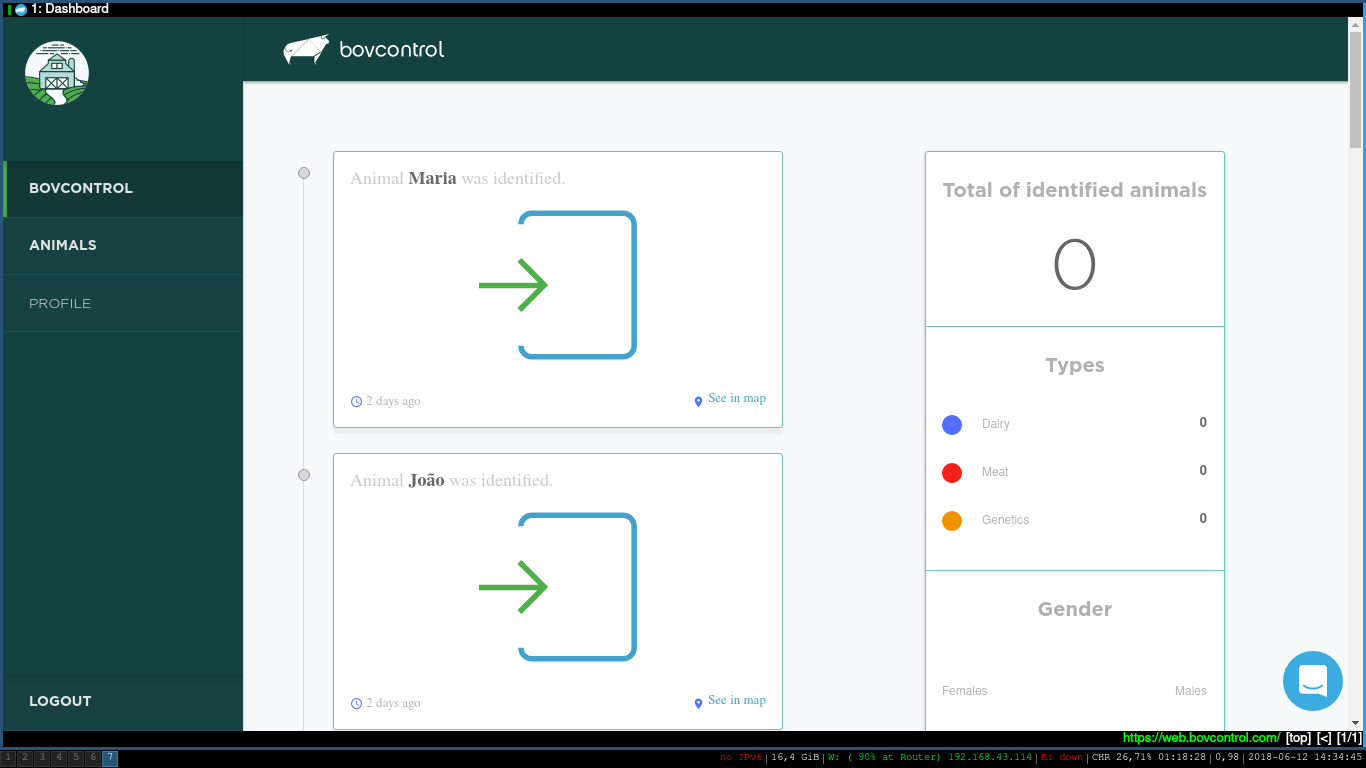
\includegraphics[width=\textwidth]{../img/bovcontrol.png}

		Fonte: Captura de tela do sistema BovControl.
	\end{center}
\end{figure}


%\begin{figure}[!h]
%\begin{center}
%\caption{BovControl versão mobile - Página inicial}
%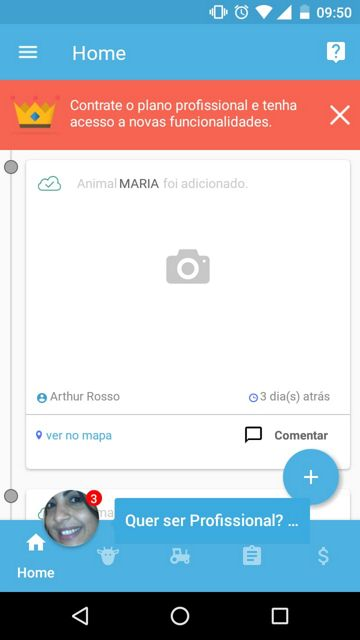
\includegraphics[width=6in]{img/bovcontrolapp1.jpg}

% % %\floatfoot{Fonte: Autoria própria.}
%\end{center}
%\end{figure}

%\begin{figure}[!h]
%\begin{center}
%\caption{BovControl versão mobile - Opções de ações}
%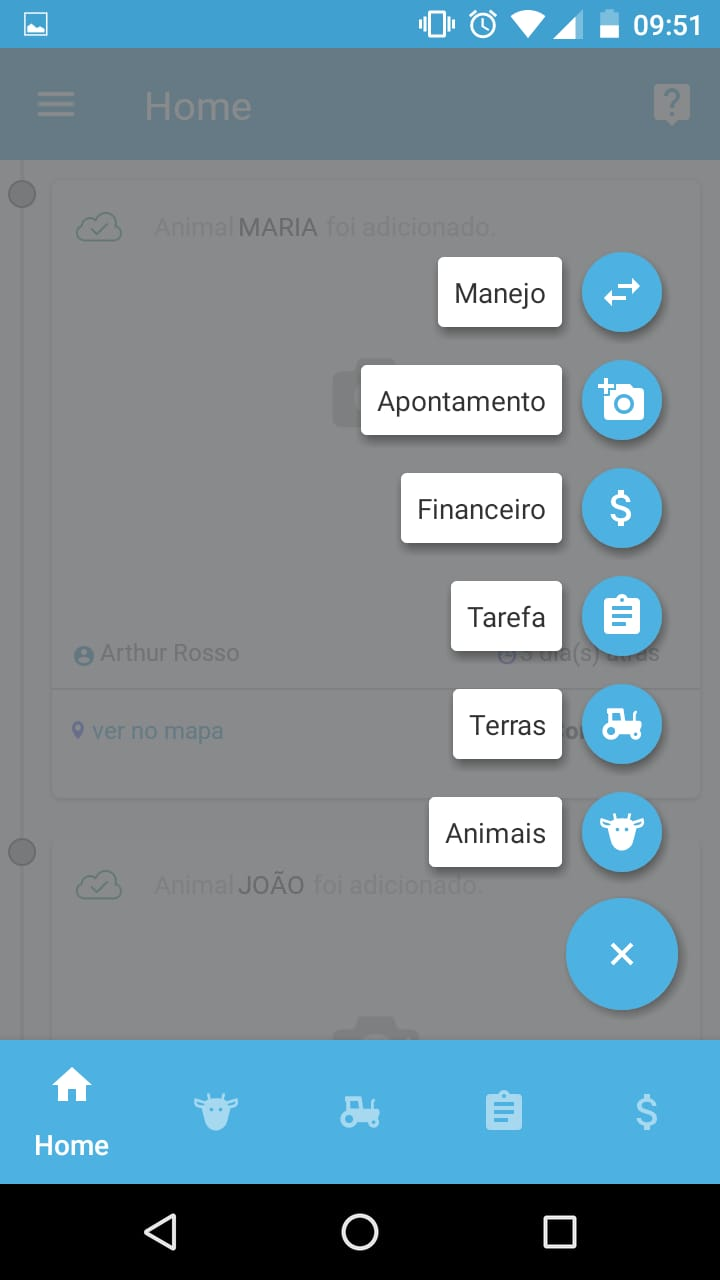
\includegraphics[width=6in]{img/bovcontrolapp2.jpeg}

% %\floatfoot{Fonte: Autoria própria.}
%\end{center}
%\end{figure}


\subsection{JETBOV}

Segundo \citeonline{jetbov16}, esse é um sistema que tem como objetivo a gestão da fazenda, da cria até a terminação, a pasto, no semi-confinamento ou confinamento, com um controle de custos com o propósito de aumento da rentabilidade.

Não possui versão gratuita, porém há uma versão de testes disponível por 21 dias, após isso é necessário realizar um orçamento individual.

O sistema apresenta 2 versões, uma web e outra mobile, a mobile é simples contendo apenas uma página com animais e um botão contendo as opções de manejo como adicionar um novo animal e sua identificação, registros sanitários como vacinações, medicações, exames, vermifugações, etc, adicionar a morte de um animal, o desmame, o parto e pesagem.

A versão web é mais completa contendo um painel de dados da fazenda, com gráficos de animais por sexo, animais por lote, peso por lote e algumas informações como número total de animais da fazenda, peso total da fazenda.

A Figura 2 apresenta uma imagem mostrando a página inicial do sistema JetBov versão web.

\begin{figure}[H]
	\begin{center}
		\caption{Página inicial da versão web do JetBov}
		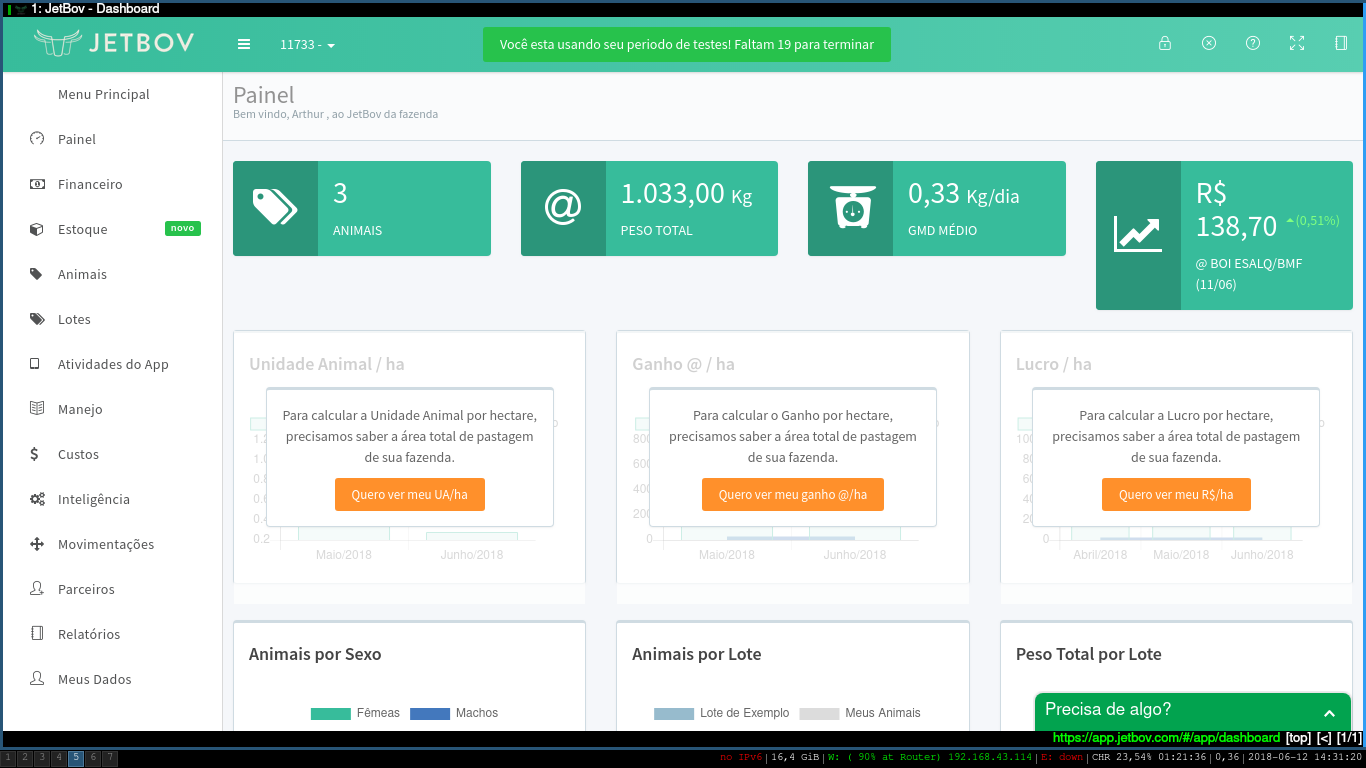
\includegraphics[width=\textwidth]{../img/jetbov.png}

		Fonte: Captura de tela do sistema JetBov.
	\end{center}
\end{figure}

%\begin{figure}[!h]
%\begin{center}
%\caption{Jetbov versão mobile - Página inicial}
%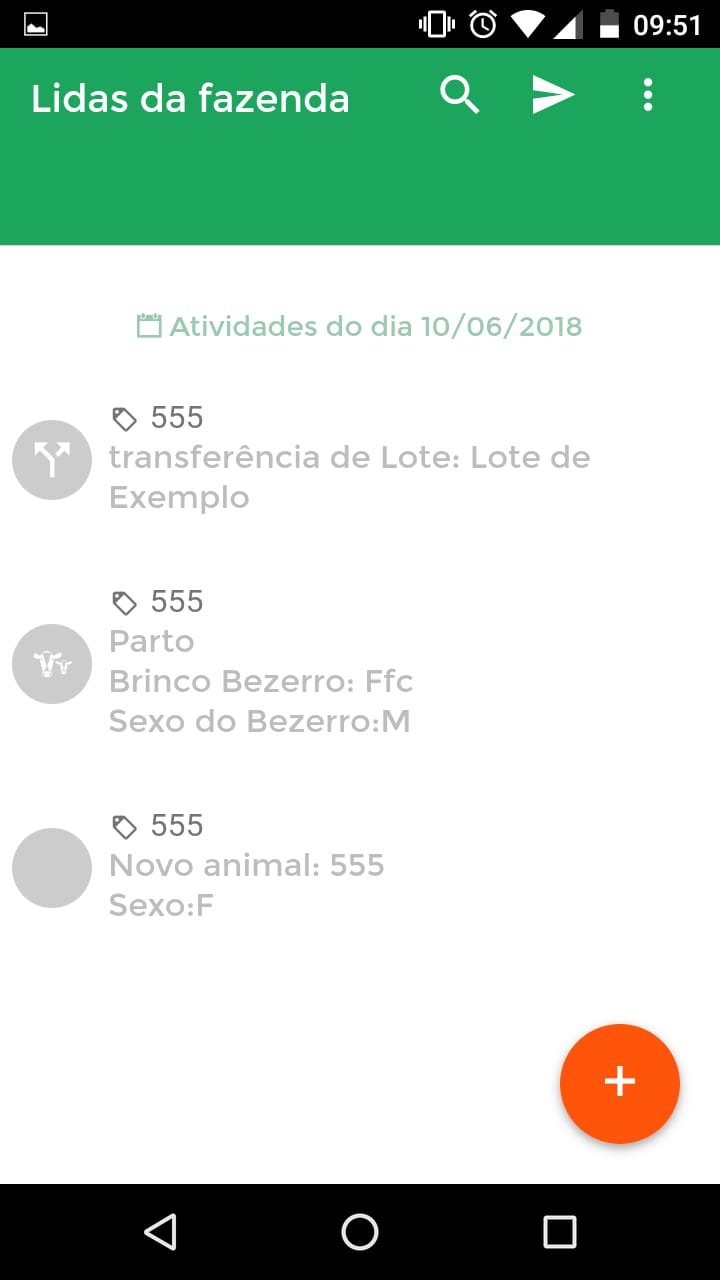
\includegraphics[width=6in]{img/jetbovapp1.jpeg}

% %\floatfoot{Fonte: Autoria própria.}
%\end{center}
%\end{figure}

%\begin{figure}[!h]
%\begin{center}
%\caption{JetBov versão mobile - Opções de ações}
%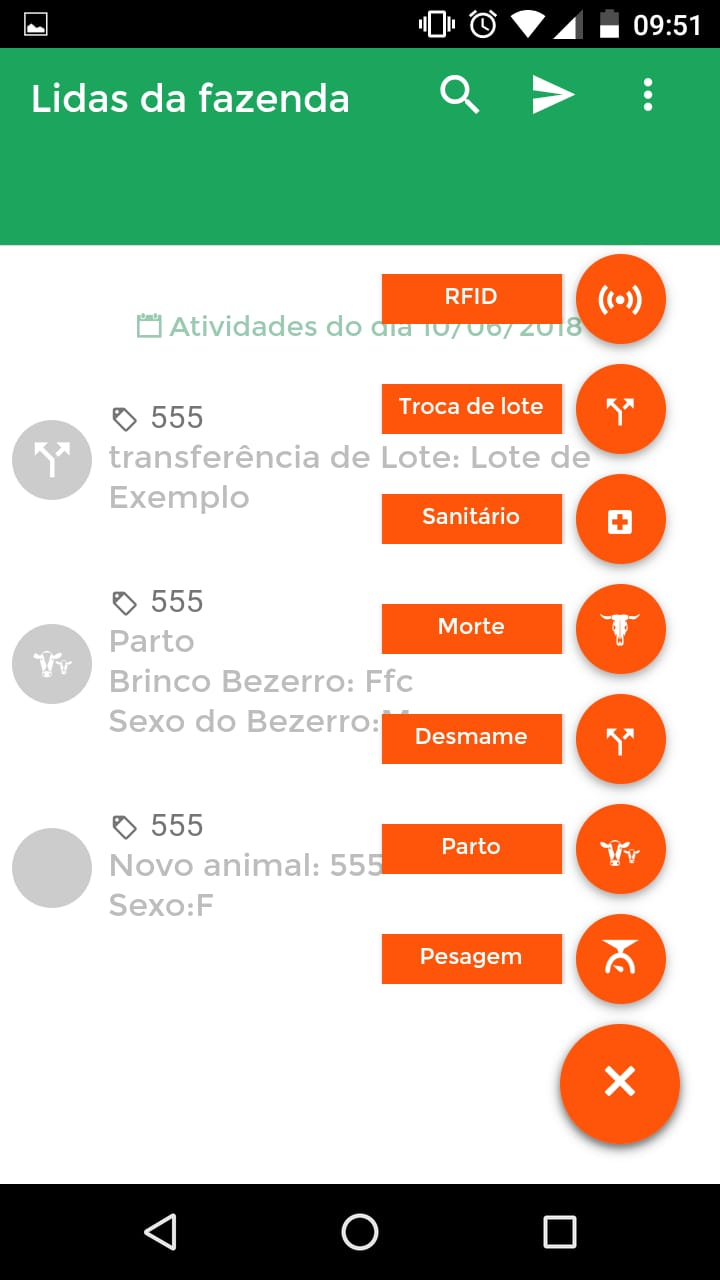
\includegraphics[width=6in]{img/jetbovapp2.jpeg}

% %\floatfoot{Fonte: Autoria própria.}
%\end{center}
%\end{figure}

\subsection{A3PECUÁRIA}

A3Pecuária é um software para gestão de animais com controle de reprodução, pesagens, vacinas e exames, controle financeiro e de estoque e compra e venda. Segundo o site do fabricante: "fornecemos importantes informações de análise de seu rebanho de maneira simples e com uma interface muito fácil de aprender, permitindo gerir seu investimento de forma a aumentar a lucratividade"  \cite{a3pecuaria16}.

Segundo \citeonline{a3pecuaria16}, são 3 tipos de planos, que variam de R\$ 29,90 a R\$ 69,90 por mês, e que gerenciam 500 animais ativos e 1 Fazenda até 3000 animais ativos e fazendas ilimitadas. Não possui versão gratuita, mas uma versão de testes por 30 dias.

Apresenta duas versões, uma web e outra mobile. A mobile, por ser simples, contém apenas a lista de animais da fazenda, o inventário, uma opção de bastão eletrônico e links para a versão web.

A versão web, por ser mais robusta e completa, apresenta uma série de possibilidades de manejos como novo lote, novo animal, nova despesa, nova receita e uma série de análise de dados com relatórios da propriedade.

A seguir, uma imagem mostrando a página inicial do sistema A3Pecuária versão web.


\begin{figure}[!h]
	\begin{center}
		\caption{Página inicial da versão web do A3Pecuária}
		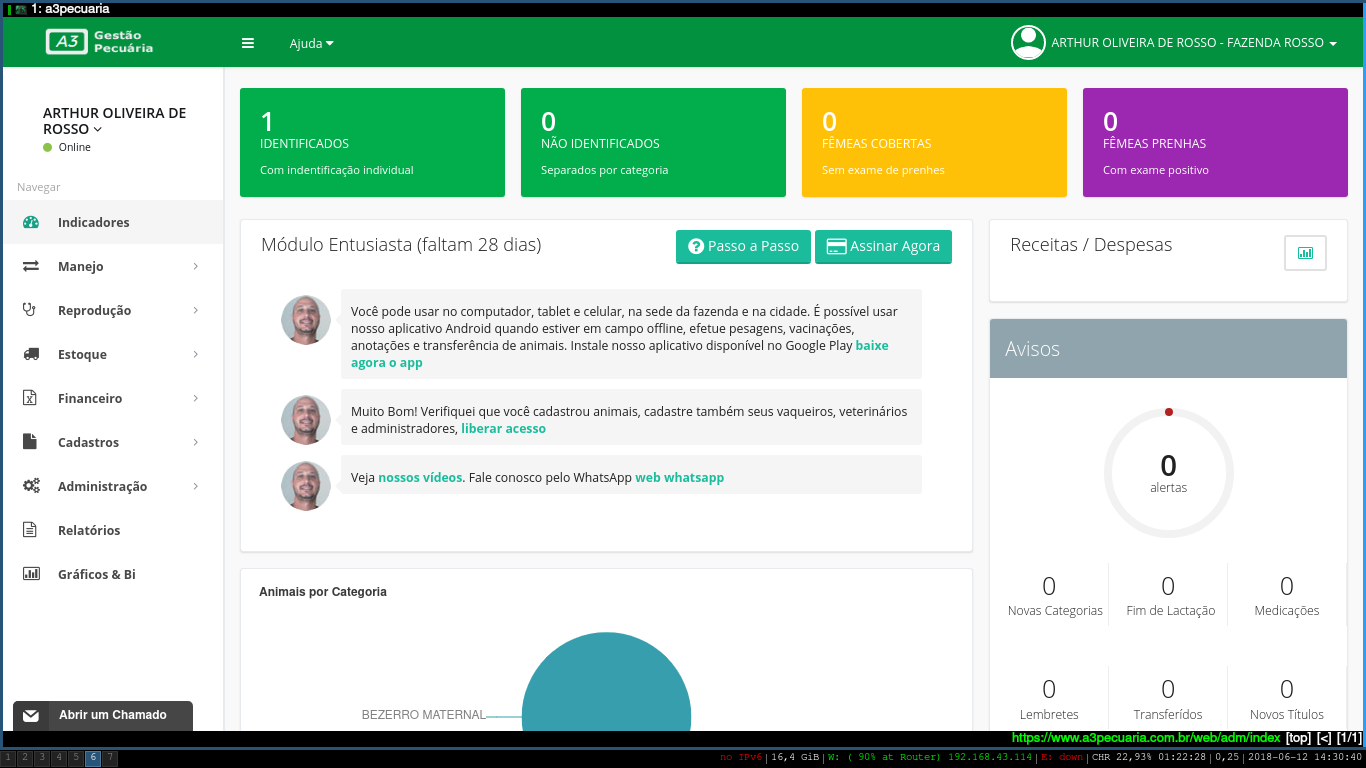
\includegraphics[width=\textwidth]{../img/a3pecuaria.png}

		Fonte: Captura de tela do sistema A3Pecuária.
	\end{center}
\end{figure}

%\begin{figure}[!h]
%\begin{center}
%\caption{A3Pecuária versão mobile - Página inicial}
%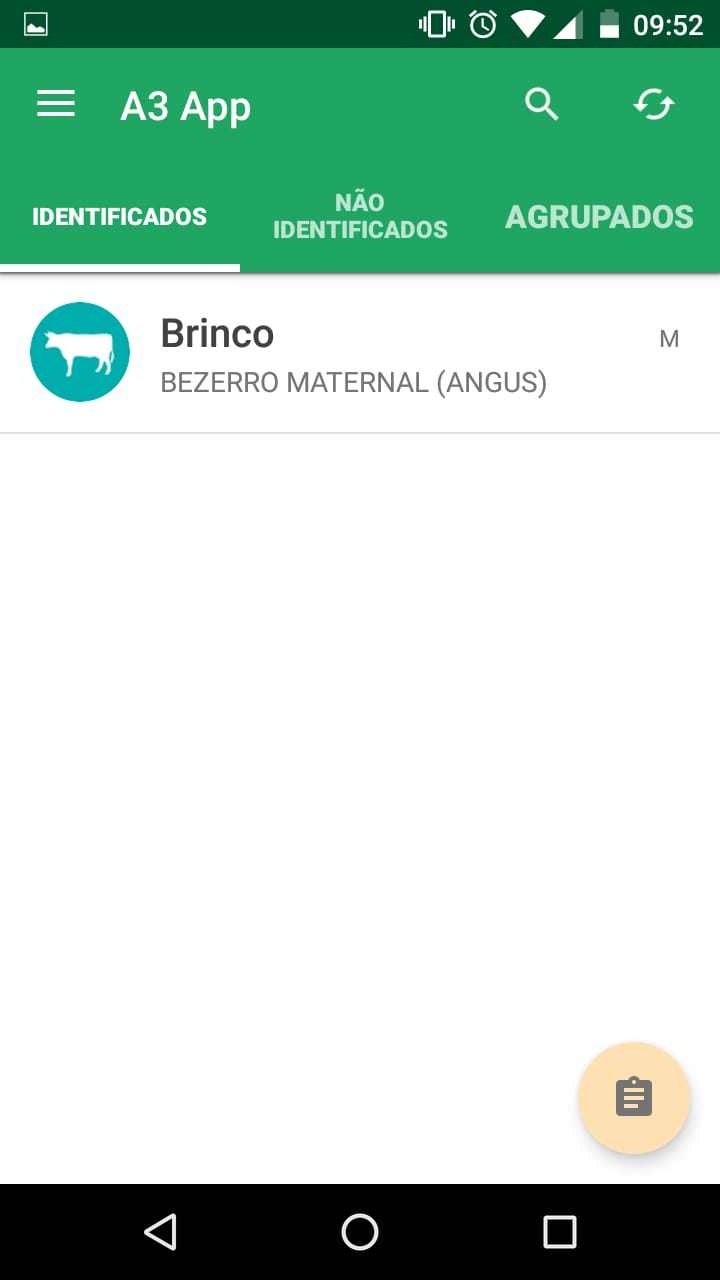
\includegraphics[width=6in]{img/a3pecuariaapp1.jpeg}

% %\floatfoot{Fonte: Autoria própria.}
%\end{center}
%\end{figure}

%\begin{figure}[!h]
%\begin{center}
%\caption{A3Pecuária versão mobile - Opções de ações}
%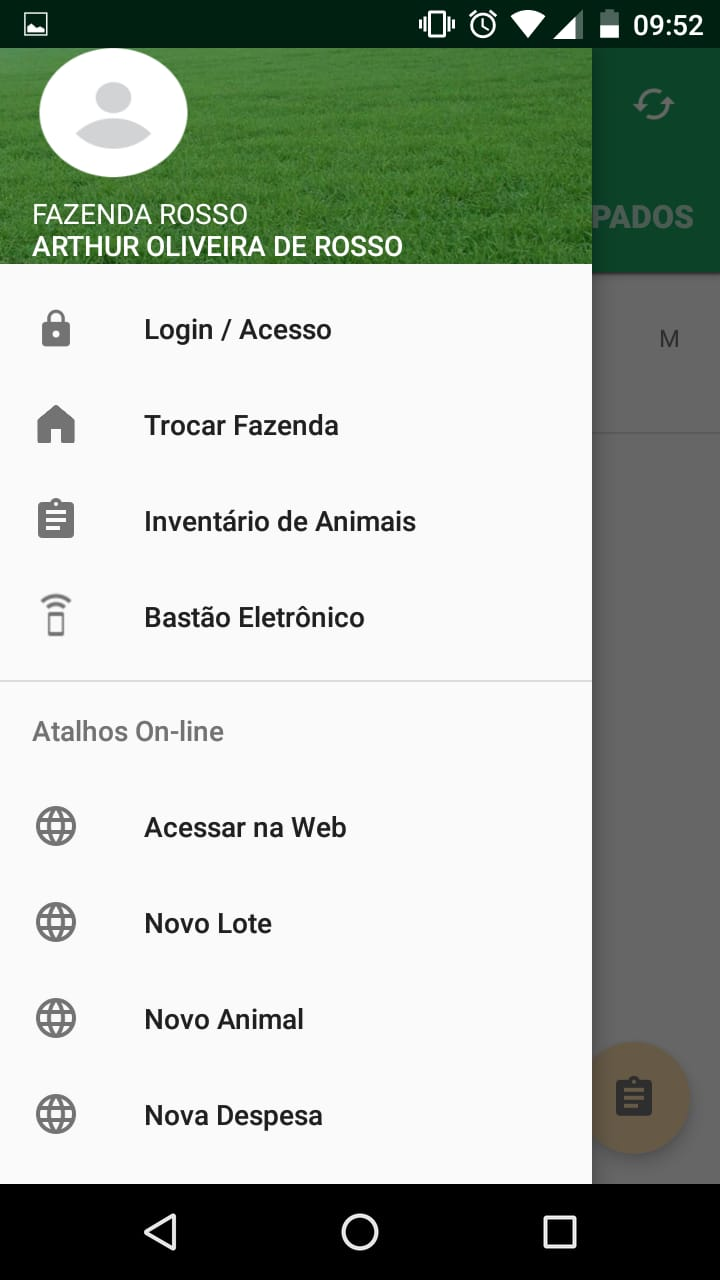
\includegraphics[width=6in]{img/a3pecuariaapp2.jpeg}

% %\floatfoot{Fonte: Autoria própria.}
%\end{center}
%\end{figure}

\subsection{ANÁLISE COMPARATIVA DOS TRABALHOS RELACIONADOS}

A partir da análise feita nas plataformas, pode-se chegar na seguinte conclusão: todas tem seu modo de operação semelhante, como criar, deletar, ler e editar as informações de um animal, e as opções de tratamento de gado (aqui chamado de manejo). As opções de estoque, que no proposto sistema é trabalhado só com medicações e a visualização de relatórios são trabalhados de maneira parecida em todos os sistemas também. Dessa maneira o sistema tem por objetivo trabalhar com estas mesmas operações, de maneira simples e sem custos.


\begin{table}[H]
	\begin{center}
		\caption{Tabela da análise dos trabalhos relacionados}
		\begin{tabular}{ | p{8cm} |  c | c | c | c |}
			\hline
			Funcionalidade & BovControl & JetBov & A3Pecuária & GoBov \\ \hline
			Gerenciamento de animais de uma propriedade & Sim & Sim & Sim & Sim \\  \hline
			Gerenciamento de medicamentos de uma propriedade & Não & Não & Sim & Sim  \\ \hline
			Gerenciamento de medicações de animais & Sim & Sim & Sim & Sim  \\ \hline
			Visualização de relatórios gerais da propriedade & Sim & Sim & Sim & Sim  \\ \hline
			Visualização de relatórios individuais de cada animal & Não & Não & Não & Sim  \\ \hline
			Possibilidade de exportar para excel & Não & Não & Não & Sim  \\ \hline
			Versão gratuita & Sim & Não & Não & Sim  \\
			\hline
		\end{tabular}
		Fonte: Autoria própria.
	\end{center}
\end{table}


\section{TECNOLOGIAS UTILIZADAS}

Esta seção tratará as tecnologias que foram utilizadas na produção do presente trabalho. Bem como os motivos de suas escolhas.

\subsection{Go}

A linguagem utilizada no \textit{back-end} é Go, uma linguagem de programação de código aberto que facilita a criação de software simples, bastante adequada para pequenos e médios projetos.

Sua utilização se justifica pela facilidade de realizar os CRUD (são as quatro operações básicas utilizadas em dados ou em bases de dados relacionais); baixa abstração o que deixa o ritmo de produção de código rápido uma vez que não é necessário pesquisar o que cada método é responsável; métodos precisos para as necessidades do problema.

\subsection{MariaDB e PostgreSQL}

Foi utilizado 2 SGBD no projeto, um local na máquina do pesquisador, o MariaDB, trata-se de um SGBD de código aberto bastante conhecido, é um \textit{fork} do MySQL, e outro para o \textit{host} remoto, para que funcione no heroku, o PostgreSQL, o "PostgreSQL é um sistema de gerenciamento de banco de dados objeto-relacional (SGBDOR) baseado no POSTGRES Versão 4.2 desenvolvido pelo Departamento de Ciência da Computação da Universidade da Califórnia em Berkeley."  \cite{postgres07}.

\subsection{HTML, CSS e JS}

Para a construção do \textit{front-end} foi utilizada a linguagem de marcação HTML que providencia a estrutura da página, para os estilos CSS. JavaScript, que é uma linguagem de programação que executa scripts no lado do cliente também foi utilizada. Também se utilizou o framework Materialize, como um facilitador da estilização das páginas HTML, assim foi possível deixa-las responsivas.

\subsection{Mustache}

Como \textit{template engine} foi utilizado o Mustache, com ele é possível mostrar nas páginas do navegador o conteúdo do banco de dados. Pelo fato de não utilizar lógica, todas as regras de negócio ficam restritas a linguagem do servidor.

\subsection{GORM}

GORM é uma biblioteca ORM para Go, ele torna desnessessária a manipulação de código SQL diretamente, facilitando assim o trânsito entre diferentes SGBD. Ele também torna o projeto mais seguro, uma vez que o deixa imune a \textit{SQL Injection}.

\subsection{Gorilla web toolkit}

Gorilla é um conjunto de pacotes para desenvolver em Go para web, entre elas as usadas foram o gorilla/mux que providencia um sofisticado acesso a rotas com váriaveis e \textit{middleware}. Outro pacote utilizado foi o gorilla/session para a manipulação das sessões, e utilizando as \textit{flashes}.
            % Fundamentação Teórica
    %
% Documento: Fundamentação Teorica
%

%\vspace{3cm}%Espaçamento entre linhas

\chapter{\textbf{DESCRIÇÃO DA SOLUÇÃO}}\label{chap:descSolucao}

Visando atender o objetivo deste trabalho de desenvolver um sistema capaz de gerenciar animais, uma solução web foi implementada. Este capítulo detalha o desenvolvimento dessa solução, partindo do modelo de requisitos do mesmo.

A análise de requisitos do presente trabalho foi realizada através de conversas com os pecuáristas do estudo de caso. Para delimitar as funcionalidades foi elaborado um diagrama de casos de uso contendo as mesmas.

\section{MODELO DE REQUISITOS}

Para a modelagem de requisitos, utilizou-se o diagrama de casos de uso porque, "ele possibilita a compreensão do comportamento externo do sistema, tornando possível ter uma visão das funcionalidades do sistema" \cite{guedes18}. Neste sentido o diagrama a seguir mostra um usuário desempenhando as funções representadas pelos casos de uso.

\begin{figure}[H]
	\begin{center}
		\caption{Diagrama de Casos de Uso do sistema}
		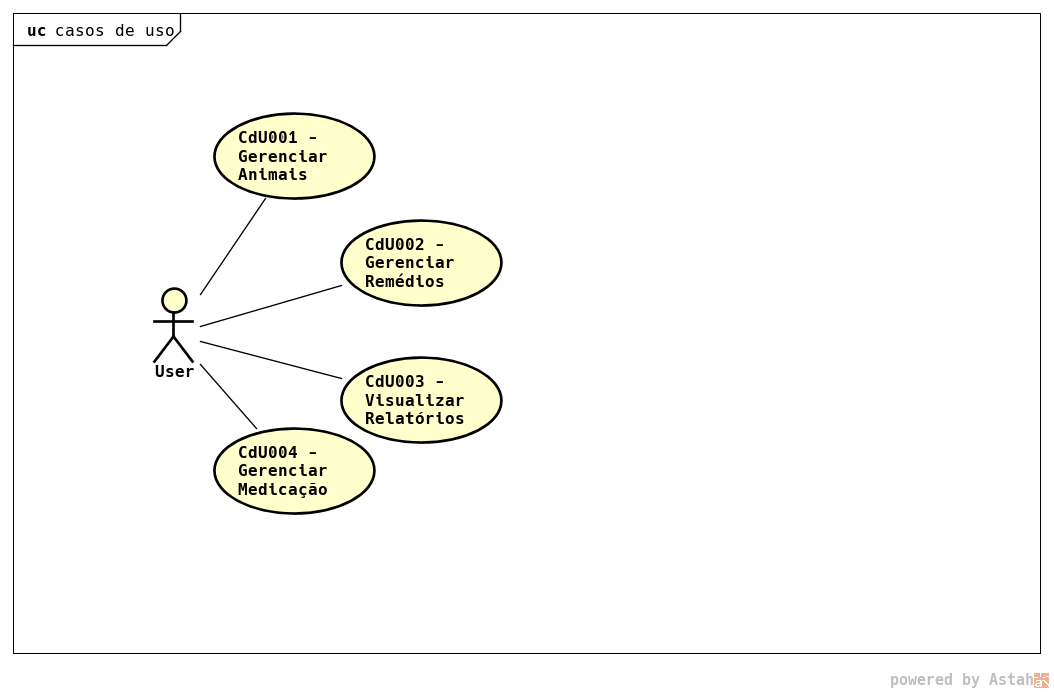
\includegraphics[width=\textwidth]{../img/casosdeuso.png}

		Fonte: Autoria própria.
	\end{center}
	\label{CdU}
\end{figure}

O caso de uso (CdU) Gerenciar Animal trata das operações realizadas com os animais, no caso, criar um animal, ler as informações dele, atualizar suas informações e deleta-lo. Os casos de uso Gerenciar Remédios e Gerenciar Medicações se referem as mesmas operações, porém, com seus respectivos objetos. O caso de uso Visualizar Relatórios se refere a visualização das informações disponibilizadas pelo sistema, como os gráficos de pesos de animais, aqui chamados de relatórios.


\subsection{\textbf{Telas do Sistema}}\label{telas}
Nesta subseção serão apresentadas as telas do sistema, quais informações elas aoresentam e quais ações elas possibilitam.

\begin{itemize}
\item IV001

A figura 5 é a tela de login do sistema. Nela, o usuário pode se autenticar ou ser direcionado para outra página com o propósito se registrar.
\begin{figure}[H]
	\begin{center}
		\caption{Login no sistema}
		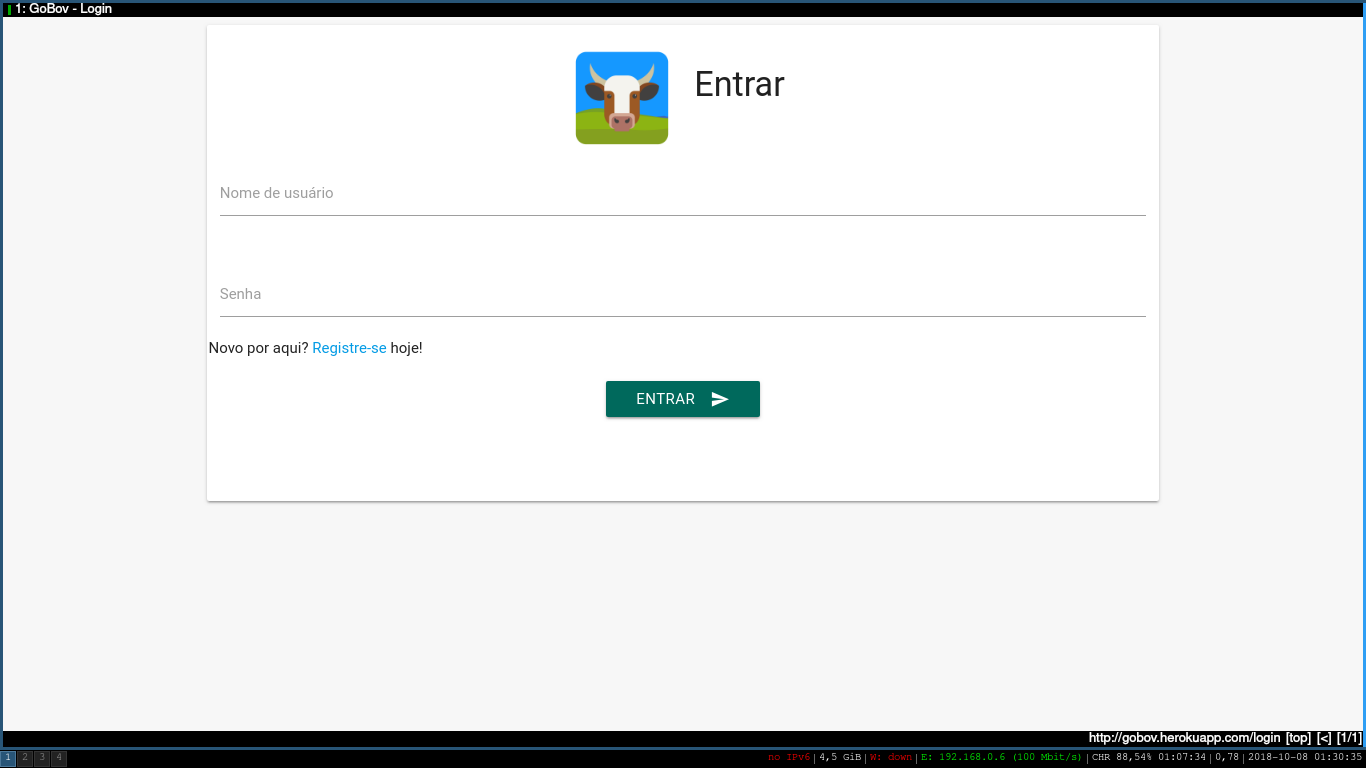
\includegraphics[width=\textwidth]{../img/prototipos/login.png}

		Fonte: Autoria própria.
	\end{center}
\end{figure}

\item IV002

A figura 6 é a tela inicial do sistema. Nela aparecem informações sobre a propriedade, como a quantidade total de animais, remédios e medicações. O usuário também pode ir para a tela de lista de animais, lista de Remédios, ou lista de medicações, ou ser direcionado para o menu, com as preferencias do usuário, nela é possível criar e deletar propósitos, tipos e raças de animais, além dos tipos de remédios.

\begin{figure}[H]
	\begin{center}
		\caption{Página inicial do sistema}
		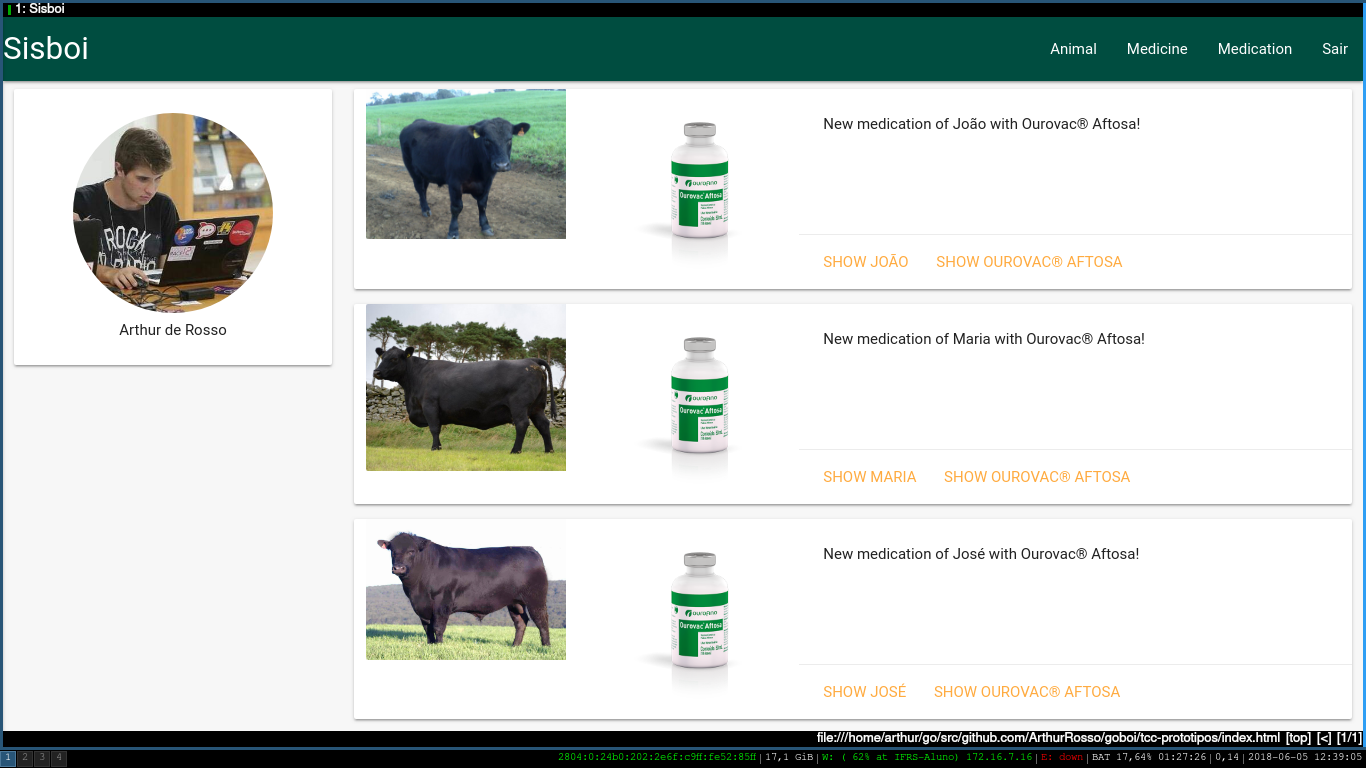
\includegraphics[width=\textwidth]{../img/prototipos/index.png}

		Fonte: Autoria própria.
	\end{center}
\end{figure}

\item IV003

A figura 7 é a página de lista de animais é apresentada a lista de animais com alguns atributos e 3 ícones, um para deletar o animal, outro para registrar uma medicação e outro para registrar um peso. É mostrada uma barra de consulta, para filtrar os resultados. O usuário pode adicionar um animal, adicionar uma medicação a um animal, pesar um animal, deletar um animal ou ir para a tela de perfil do animal.
\begin{figure}[H]
	\begin{center}
		\caption{Página do animais}
		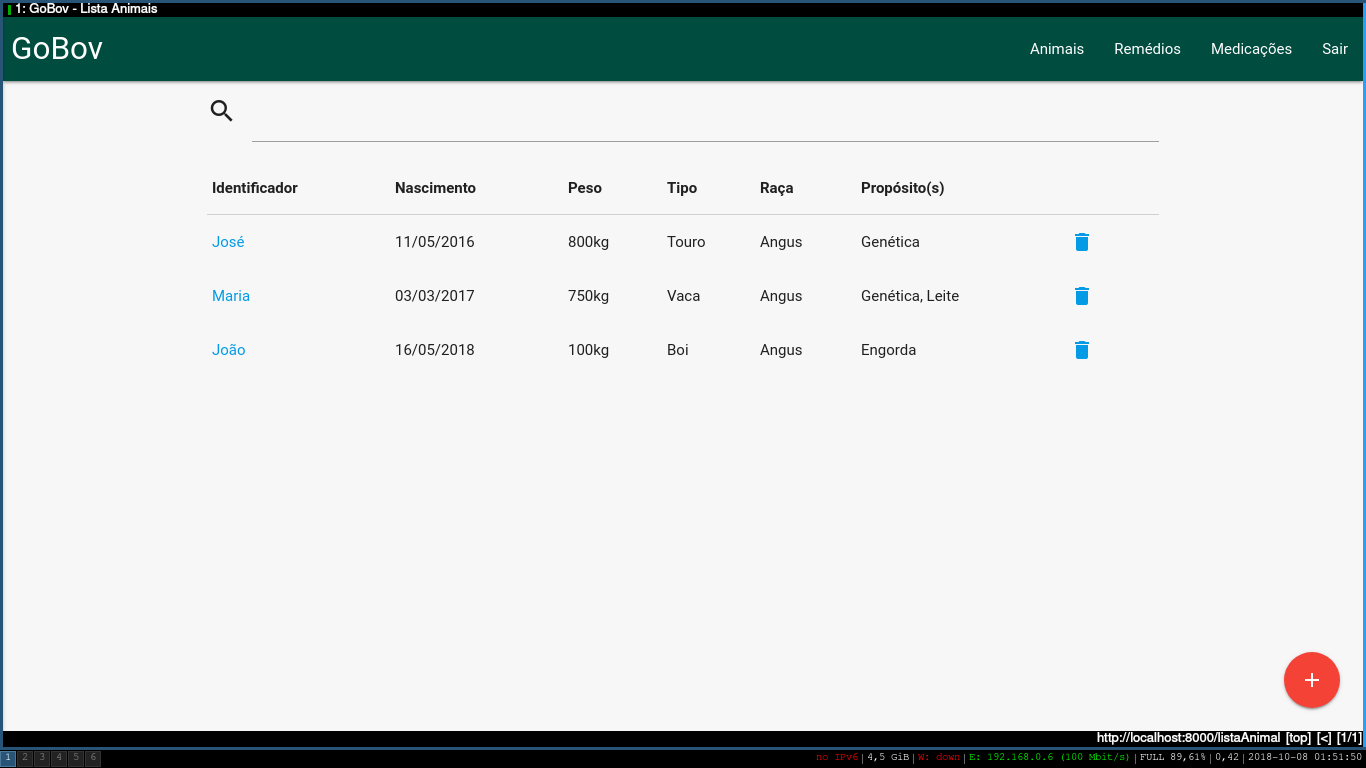
\includegraphics[width=\textwidth]{../img/prototipos/listaAnimal.png}

		Fonte: Autoria própria.
	\end{center}
\end{figure}

\item IV004

A figura 8 é a página de adicionar animal. O usuário insere as informações do animal e solicita salvar, após isso ele é direcionado para a página de perfil do animal recém adicionado.
\begin{figure}[H]
	\begin{center}
		\caption{Página de adicionar animal}
		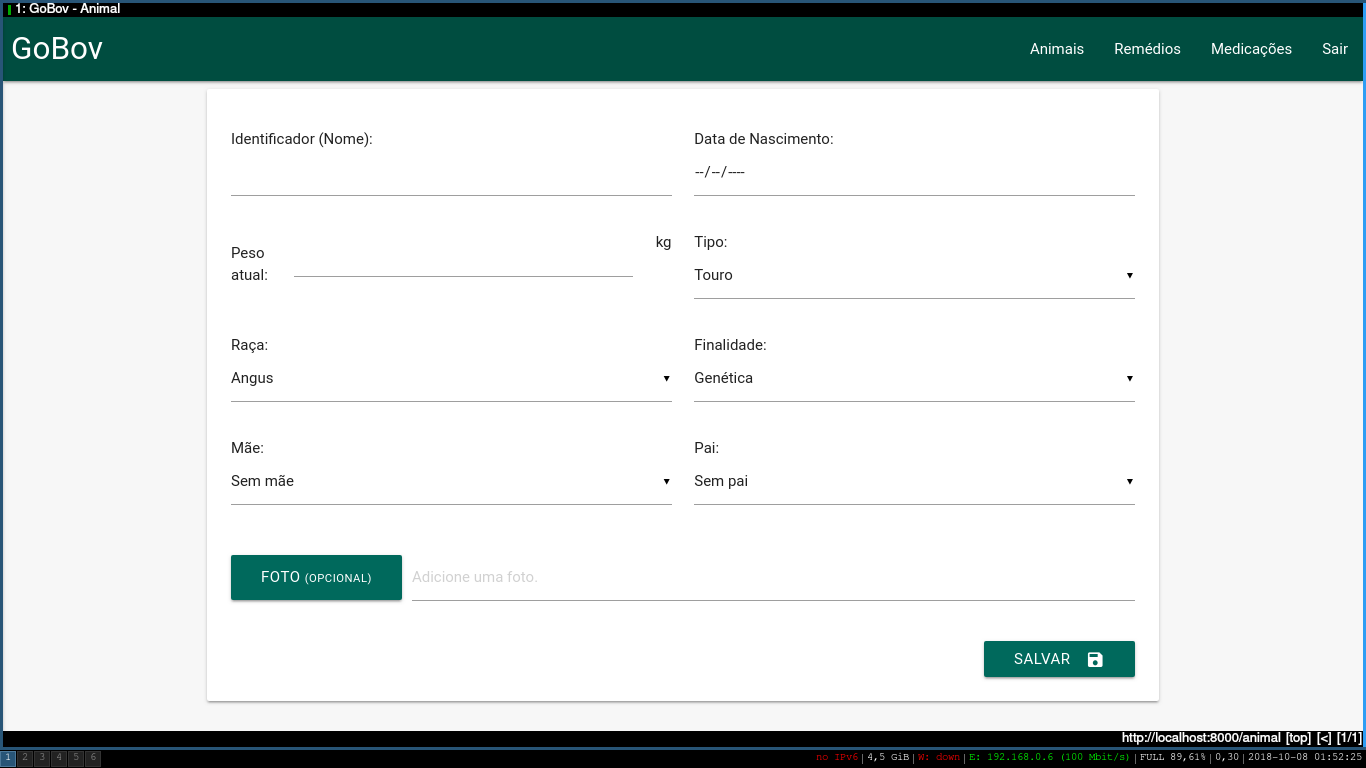
\includegraphics[width=\textwidth]{../img/prototipos/addAnimal.png}

		Fonte: Autoria própria.
	\end{center}
\end{figure}


\item IV005

A figura 9 é a página de lista de remédios, é mostrado as informações dos remédios do usuário. Na página o usuário pode adicionar, deletar ou editar um remédio.
\begin{figure}[H]
	\begin{center}
		\caption{Página de remédios}
		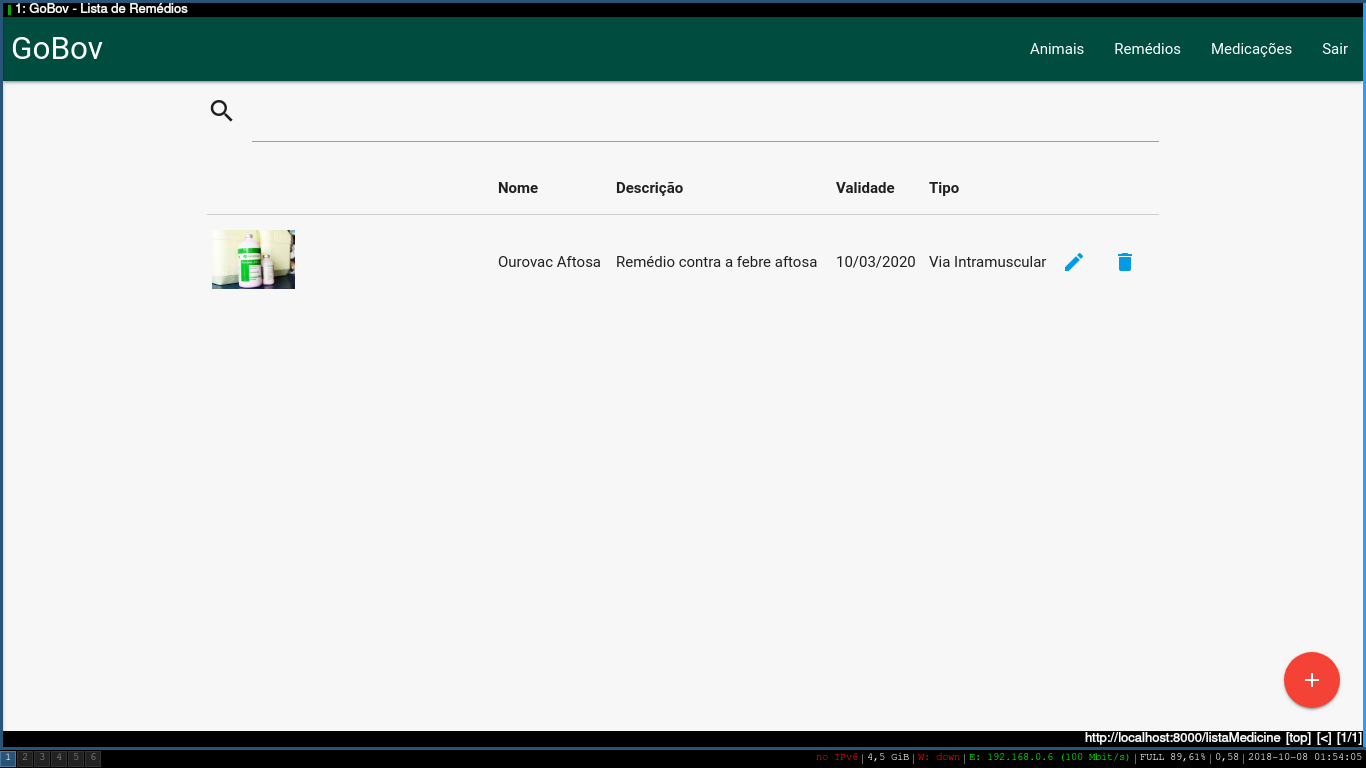
\includegraphics[width=\textwidth]{../img/prototipos/listaRemedio.png}

		Fonte: Autoria própria.
	\end{center}
\end{figure}

\item IV006

A figura 10 é a página de adicionar remédio. O usuário insere as informações do remédio e solicita salvar, após isso ele é direcionado para a página da lista de remédios.
\begin{figure}[H]
	\begin{center}
		\caption{Página de adicionar remédio}
		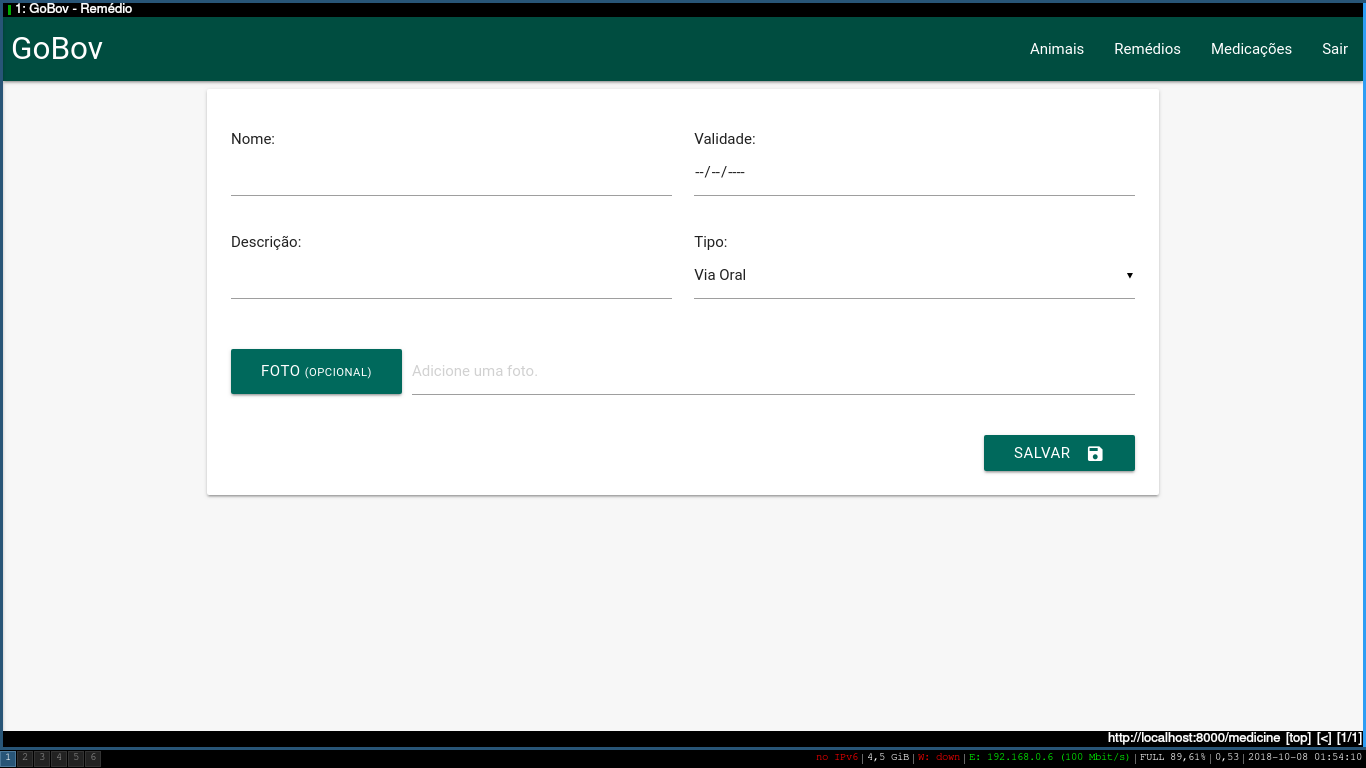
\includegraphics[width=\textwidth]{../img/prototipos/addRemedio.png}

		Fonte: Autoria própria.
	\end{center}
\end{figure}


\item IV007

A figura 11 é a página de lista de medicações, é apresentado as medicações realizadas com uma descrição, a data da realização, a lista de animais medicados e os remédios utilizados. Nela, o usuário pode adicionar ou deletar uma medicação.
\begin{figure}[H]
	\begin{center}
		\caption{Página de medicações}
		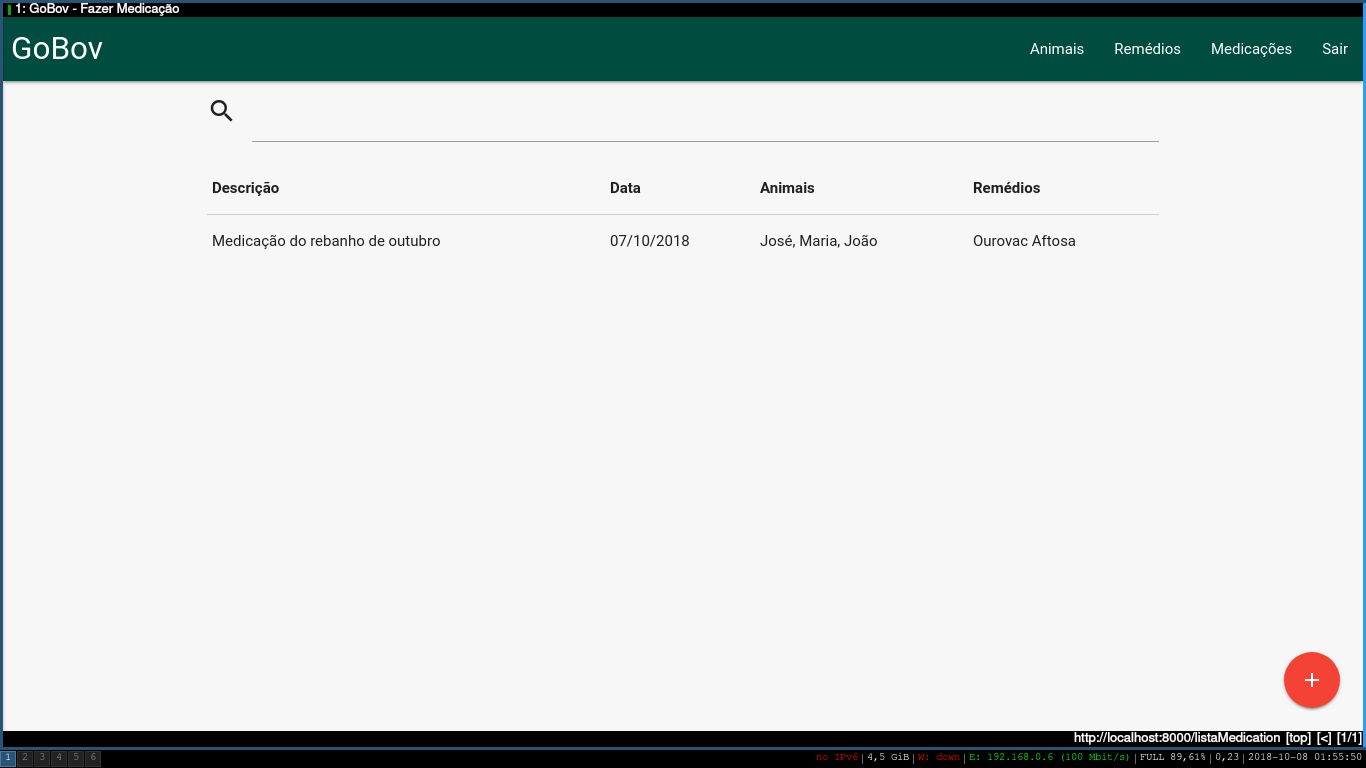
\includegraphics[width=\textwidth]{../img/prototipos/listaMedicacao.png}

		Fonte: Autoria própria.
	\end{center}
\end{figure}

\item IV008

A figura 12 é a página de adicionar medicação. Nela o usuário insere uma descrição, a data que a medicação ocorreu, os animais medicados e os remédios utilizados.
\begin{figure}[H]
	\begin{center}
		\caption{Página de adicionar medicação}
		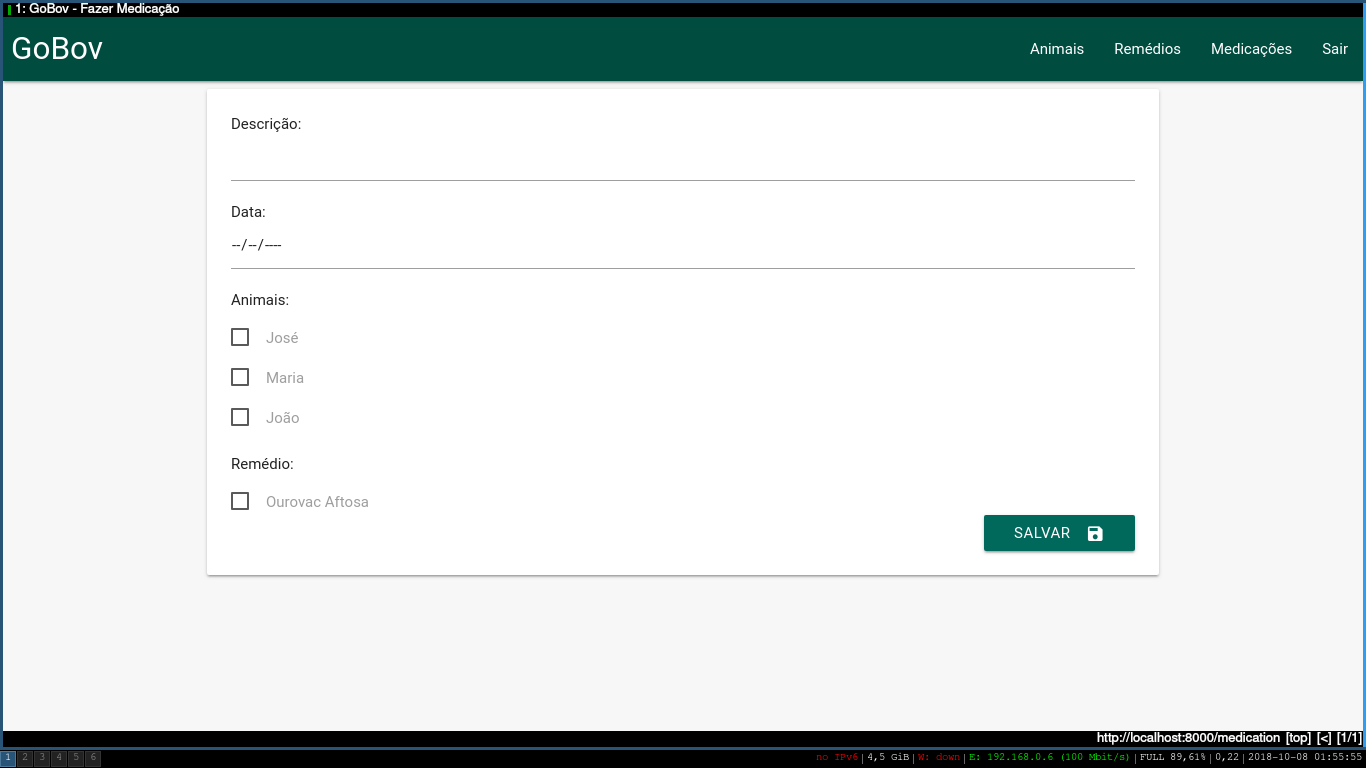
\includegraphics[width=\textwidth]{../img/prototipos/addMedicacao.png}

		Fonte: Autoria própria.
	\end{center}
\end{figure}

\item IV009

A figura 13 é a página de perfil do animal. Nela, são apresentadas todas as informações do animal, inclusive um histórico do que aconteceu com o animal. O usuário pode editar, consultar detalhes, gerenciar uma pesagem do animal ou consultar relatórios individuais do animal.
\begin{figure}[H]
	\begin{center}
		\caption{Página de perfil do animal}
		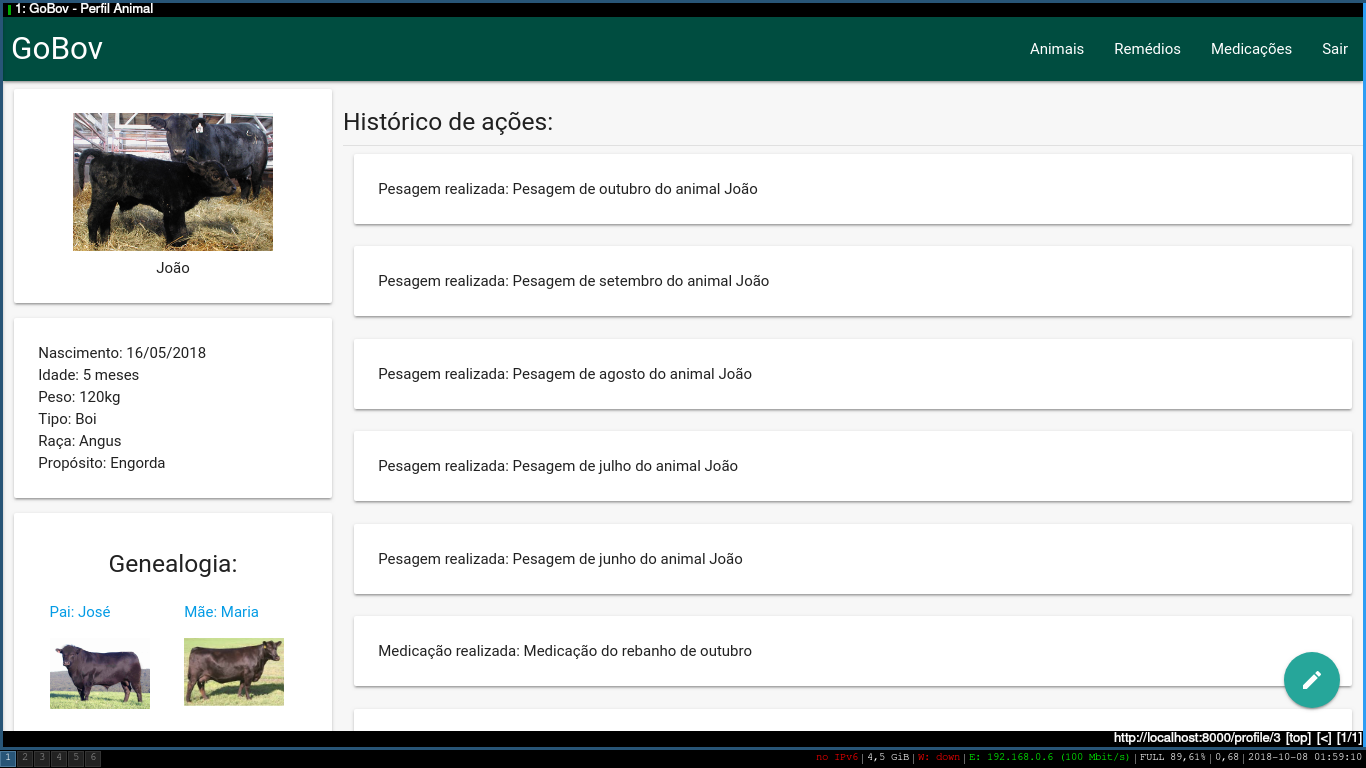
\includegraphics[width=\textwidth]{../img/prototipos/perfil.png}

		Fonte: Autoria própria.
	\end{center}
\end{figure}


\item IV010

A figura 14 é a página de edição do animal. Nela o usuário pode editar as informações básicas do animal.
\begin{figure}[]
	\begin{center}
		\caption{Página de edição do animal}
		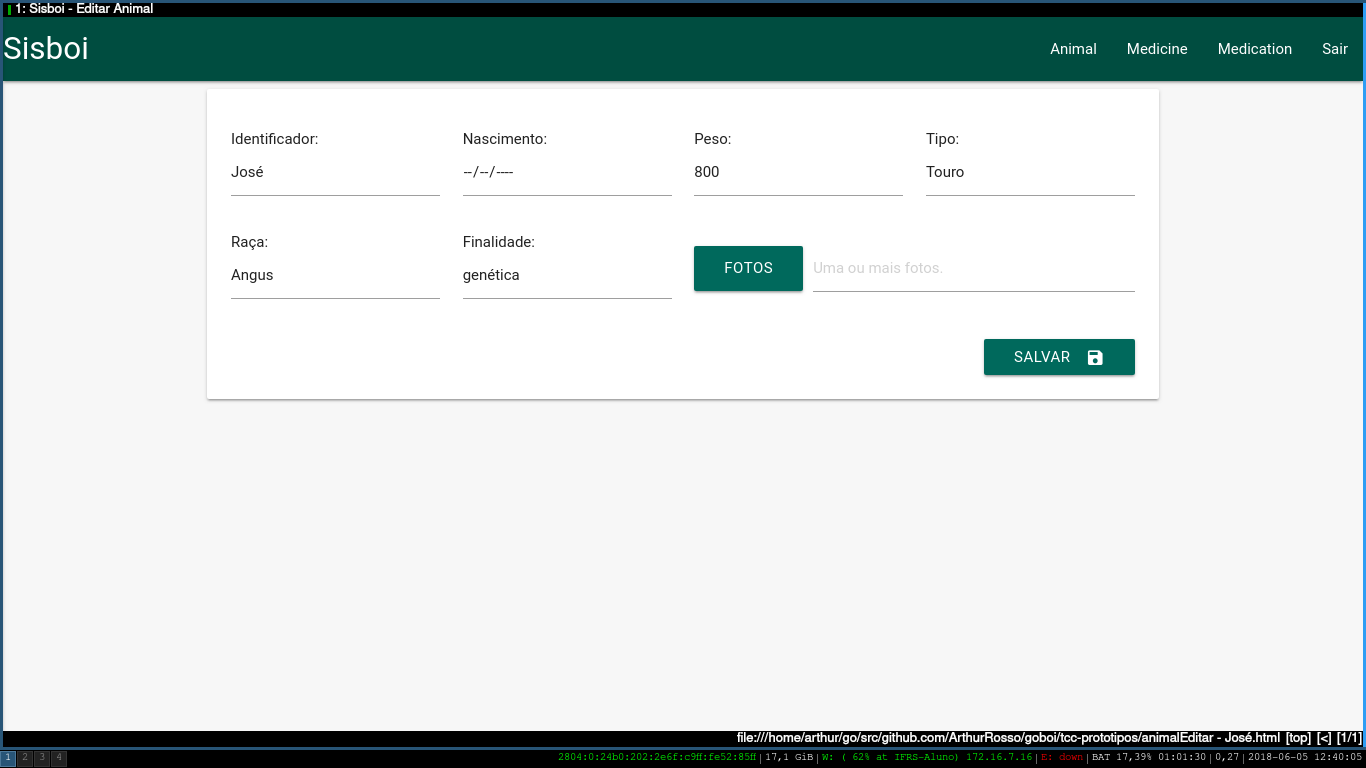
\includegraphics[width=\textwidth]{../img/prototipos/editar.png}

		Fonte: Autoria própria.
	\end{center}
\end{figure}

\newpage
\item IV011

A figura 15 é a página de pesagem. É apresentada a lista de pesagens do animal e o usuário pode gerenciar o peso de um animal.
\begin{figure}[H]
	\begin{center}
		\caption{Página de pesagem do animal}
		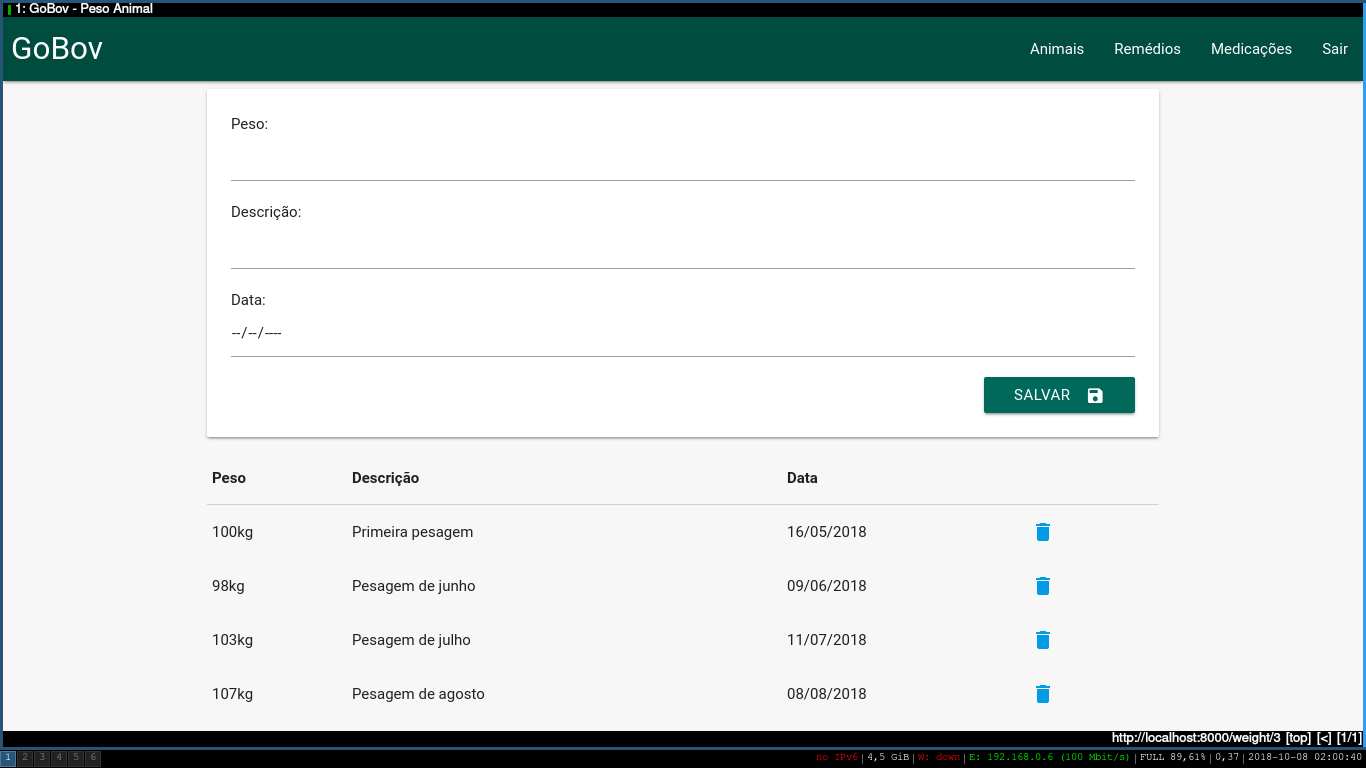
\includegraphics[width=\textwidth]{../img/prototipos/addPeso.png}

		Fonte: Autoria própria.
	\end{center}
\end{figure}

\item IV012

A figura 16 é a página de relatórios individuais do animal a qual é apresentado o gráfico do peso do animal ao longo do tempo.
\begin{figure}[H]
	\begin{center}
		\caption{Página de pesagem do animal}
		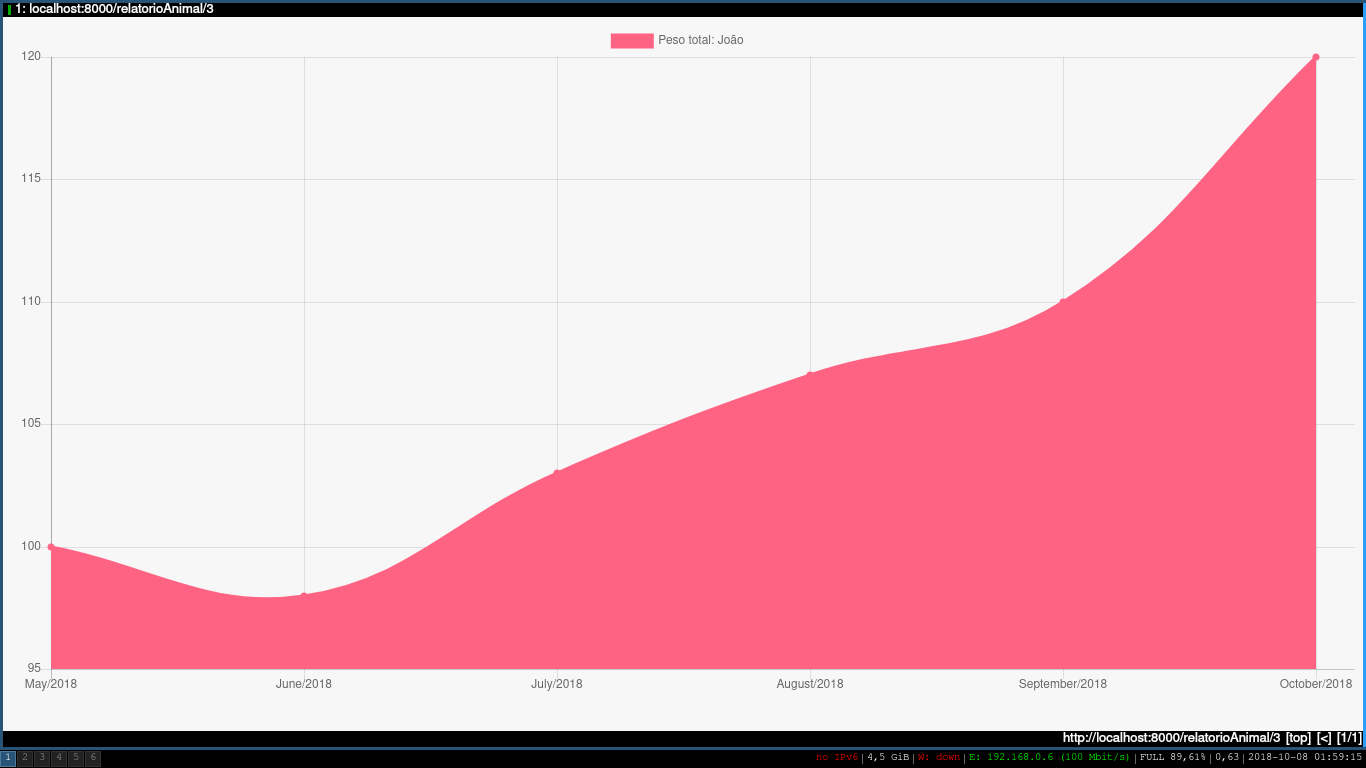
\includegraphics[width=\textwidth]{../img/prototipos/relatorio.png}

		Fonte: Autoria própria.
	\end{center}
\end{figure}

\end{itemize}

\section{MODELO ENTIDADE RELACIONAMENTO}

O diagrama a seguir mostra o modelo Entidade Relacionamento (ER), que caracteriza a abstração do banco de dados representando a relação do animal com o usuário, com a foto, com o peso, com o propósito, com a raça, com o tipo, e com a remédio, na qual é chamada de medicação. Por sua vez, o remédio também tem uma relação além da medicação, que é o tipo.

\begin{figure}[H]
	\begin{center}
		\caption{Modelo ER}
		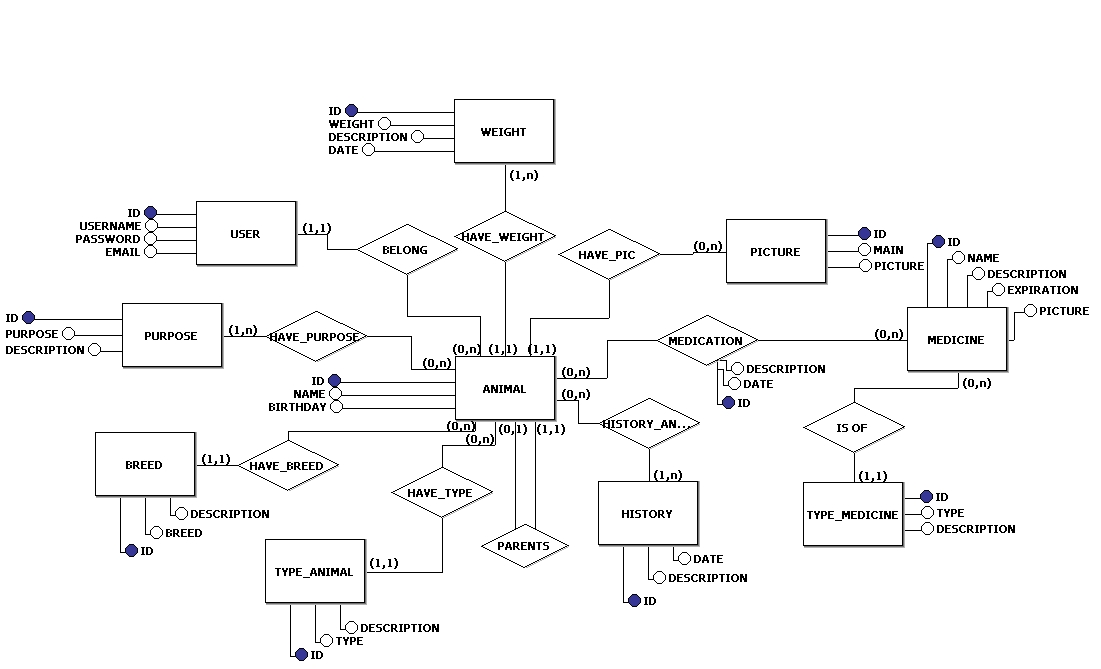
\includegraphics[width=\textwidth]{../img/erdoboi.jpg}

		Fonte: Autoria própria.
	\end{center}
	\label{er}
\end{figure}
            % Descrição da Solução
    %
% Documento: Resultados
%

%\vspace{3cm}%Espaçamento entre linhas

\chapter{\textbf{CONCLUSÃO}}\label{chap:conclusao}

Iniciou-se o trabalho com o problema da organização dos pecuáristas, assim o objeto geral era implementar um sistema capaz de auxiliá-los com a administração do gado. Para que se atenda de forma completa o objetivo geral do trabalho, foram definidos objetivos específicos, tais como:

\begin{itemize}
	\item Escolher as tecnologias a serem utilizadas no sistema:
	\newline
	Foram escolhidas a linguagem de programação Go, o banco de dados MariaDB e HTML, CSS e JS para compor as páginas no lado do cliente. Assim pode-se notar que este objetivo foi concluído com sucesso.

	\item Pesquisar as necessidades dos pecuaristas e de que maneira o sistema pode auxiliá-los com a identificação das informações relevantes sobre o ciclo de vida do animal bovino:
	\newline
	Na metodologia é explicado que houveram conversas e entrevistas com pecuaristas ao longo do ano para completar esse objetivo.	Na análise dos trabalhos relacionados foi realizada uma comparação para identificar quais são os pontos básicos de um sistema gerenciador bovino e quais pontos os usuários se encontram desamparados, para tanto foram feitas perguntas aos participantes do estudo de caso. Esse objetivo também foi concluído com sucesso.

	\item Modelar o sistema:
	\newline
	A modelagem pode ser observada na especificação dos casos de uso (Apêndice \ref{ap:especCdU}),  nos diagramas de casos de uso (\ref{CdU}), atividades (Apêndice \ref{ap:ativ}) e no modelo ER (\ref{er}). Por causa disso, o objetivo foi concluído com êxito.


	\item Realizar pesquisas de sistemas relacionados para identificar pontos onde há um nicho de mercado:
	\newline
	Dentre os sistemas pesquisados na análise dos trabalhos relacionados foi identificado que somente o presente sistema é totalmente gratuíto, é o único a possibilitar a visualização de relatórios individuais para cada animal e a exportação para planilhas excel.

	\item Implementar o sistema:
	\newline
	Através do uso das tecnologias apresentadas na seção \ref{tec} foi possível implementar o sistema das telas da subseção \ref{telas} para completar esse objetivo.

	\item Avaliar o sistema na realidade dos pecuaristas:
	\newline
	Para atender este objetivo foi feita uma entrevista com um usuário do sistema (Apêndice \ref{ap:entre}), nele foram feitas perguntas quanto a usabilidade e a experiência no sistema, com as respostas foi possível constatar que o usuário considerou as funcionalidades do trabalho úteis e conseguiu realizar suas operações de manejo no sistema, o que corrobora o cumprimento dos objetivos do trabalho.
\end{itemize}

O trabalho foi apresentado em eventos como VI IFCITEC, a Feira de Ciência e Inovação Tecnológica, realizado no Campus Canoas do Instituto Federal de Educação, Ciência e Tecnologia (IFRS) e a ENPEX, Salão de Ensino, Pesquisa e Extensão do IFRS. Nos eventos foram constatados algumas funcionalidades que ficarão como proposta de trabalhos futuros como: a possibilidade de inserir no sistema o tipo de nutrição do animal e fazer um aplicativo para que se possa utilizar o sistema sem necessitar o acesso a internet visto que nem todas as propriedades tem acesso a mesma.
             % Resultados

    % Elementos pós textuais
    \postextual
    %
% Documento: Referências Bibliográficas
%

\bibliography{refbase}    % Geração automática das referências por meio do arquivo 'refbase.bib'
        % Referências
    %
% Documento: Apêndices
%

\begin{apendicesenv}

\chapter{ESPECIFICAÇÕES DOS CASOS DE USO}

\begin{table}[!h]
	\begin{center}
		\caption{Especificação do caso de uso Gerenciar Animais}
		\begin{tabular}{ | l |  p{10cm} |}
			\hline
			Código e Nome do Caso de Uso & CdU001 - Gerenciar Animais \\ \hline
			Ator Primário: & Usuário \\
			Ator Secundário: & Não se aplica \\ \hline
			Fluxo Principal de Eventos & P1. O usuário solicita consultar os animais. \\
						   & P2. O sistema apresenta a tela de animais. (IV003) (A1) (A2) \\
						   & P3. O usuário solicita ver um animal em específico. \\
						   & P4. O sistema apresenta a tela de perfil do animal. (IV006) (A3) (A4)  \\
						   & P5. O caso de uso se encerra. \\ \hline
			Fluxo Alternativo:         & A1.1. Em P2 o usuário insere as informações de um animal no formulário e solicita salvá-las. \\
			A1. Adicionar animal       & A1.2. O sistema salva o animal. \\
						   & A1.3. Retorna ao P2. \\ \hline
			Fluxo Alternativo:         & A2.1. Em P2 o usuário tem a intenção de deletar um animal. \\
			A2. Deletar animal         & A2.2. O sistema apaga o animal selecionado. \\
						   & A2.3. Retorna ao P2. \\ \hline
			Fluxo Alternativo:         & A3.1. Em P4 o usuário decide editar animal. \\
			A3. Editar animal          & A3.2. O sistema apresenta a tela de editar animal. (IV007) \\
						   & A3.3. O usuário insere as novas informações do animal. \\
						   & A3.4. O sistema salva essas informações. \\
						   & A3.5. Retorna ao P4. \\ \hline
			Fluxo Alternativo:         & A4.1. Em P4 o decide adicionar uma nova pesagem do animal. \\
			A4. Adicionar peso         & A4.2. O sistema apresenta a tela de adicionar pesagem. (IV008) \\
						   & A4.3. O usuário insere as novas informações de peso do animal. \\
						   & A4.4. O sistema salva essas informações. \\
						   & A4.3. Retorna ao P4. \\ \hline
			Fluxo Alternativo:         & A5.1. Em P4 o usuário decide consultar detalhes do animal. \\
			A5. Consultar Detalhes     & A5.2. O sistema apresenta a tela de detalhes do animal. \\
						   & A5.3. Retorna ao P4. \\
			\hline
		\end{tabular}
		Fonte: Autoria própria.
	\end{center}
\end{table}

\newpage

\begin{table}[!h]
	\begin{center}
		\caption{Especificação do caso de uso Gerenciar Remédios}
		\begin{tabular}{ | l |  p{10cm} |}
			\hline
			Código e Nome do Caso de Uso & CdU002 - Gerenciar Remédios \\ \hline
			Ator Primário: & Usuário \\
			Ator Secundário: & Não se aplica \\ \hline
			Fluxo Principal de Eventos & P1. O usuário solicita consultar os remédios. \\
						   & P2. O sistema apresenta a tela de remédios. (IV004) (A1) (A2) (A3) \\
						   & P3. O caso de uso se encerra. \\ \hline
			Fluxo Alternativo:         & A1.1. Em P2 o usuário insere as informações de um remédio no formulário e solicita salvá-las. \\
			A1. Adicionar remédio      & A1.2. O sistema salva o remédio. \\
						   & A1.3. Retorna ao P2. \\ \hline
			Fluxo Alternativo:         & A2.1. Em P2 o usuário resolve deletar um remédio. \\
			A2. Deletar remédio        & A2.2. O sistema apaga o remédio selecionado. \\
						   & A2.3. Retorna ao P2. \\ \hline
			Fluxo Alternativo:         & A3.1. Em P2 o usuário decide editar um remédio. \\
			A3. Editar remédio         & A3.2. O sistema apresenta a tela de editar remédio. \\
						   & A3.3. O usuário insere as novas informações do remédio. \\
						   & A3.4. O sistema salva essas informações. \\
						   & A3.5. Retorna ao P2. \\
			\hline
		\end{tabular}
		Fonte: Autoria própria.
	\end{center}
\end{table}

\begin{table}[!h]
	\begin{center}
		\caption{Especificação do caso de uso Visualizar Relatórios}
		\begin{tabular}{ | l |  p{10cm} |}
			\hline
			Código e Nome do Caso de Uso & CdU003 - Visualizar Relatórios \\ \hline
			Ator Primário: & Usuário \\
			Ator Secundário: & Não se aplica \\ \hline
			Fluxo Principal de Eventos & P1. O usuário solicita consultar os relatórios. \\
						   & P2. O sistema apresenta a tela de relatórios da fazenda. \\
						   & P3. O caso de uso se encerra. \\
			\hline
		\end{tabular}
		Fonte: Autoria própria.
	\end{center}
\end{table}

\newpage

\begin{table}[!h]
	\begin{center}
		\caption{Especificação do caso de uso Gerenciar Medicação}
		\begin{tabular}{ | l |  p{10cm} |}
			\hline
			Código e Nome do Caso de Uso & CdU004 - Gerenciar Medicação \\ \hline
			Ator Primário: & Usuário \\
			Ator Secundário: & Não se aplica \\ \hline
			Fluxo Principal de Eventos & P1. O usuário solicita consultar medicação. \\
						   & P2. O sistema apresenta a tela de medicação. (IV005) (A1) (A2) (A3) \\
						   & P3. O caso de uso se encerra. \\ \hline
			Fluxo Alternativo:         & A1.1. Em P2 o usuário insere as informações de uma medicação e solicita salvá-las. \\
			A1. Adicionar medicação    & A1.2. O sistema salva a medicação. \\
						   & A1.3. Retorna ao P2. \\ \hline
			Fluxo Alternativo:         & A1.1. Em P2 o usuário resolve deletar uma medicação. \\
			A2. Deletar medicação      & A2.2. O sistema apaga a medicação selecionada. \\
						   & A2.3. Retorna ao P2. \\ \hline
			Fluxo Alternativo:         & A3.1. Em P2 o usuário decide editar uma medicação. \\
			A3. Editar medicação       & A3.2. O sistema apresenta a tela de editar medicação. \\
						   & A3.3. O usuário insere as novas informações da medicação. \\
						   & A3.4. O sistema salva essas informações. \\
						   & A3.5. Retorna ao P2. \\
			\hline
		\end{tabular}
		Fonte: Autoria própria.
	\end{center}
\end{table}


\chapter{DIAGRAMAS DE ATIVIDADE}
\begin{figure}[H]
	\begin{center}
		\caption{Diagrama da Atividade de Gerenciar Animal parte 1}
		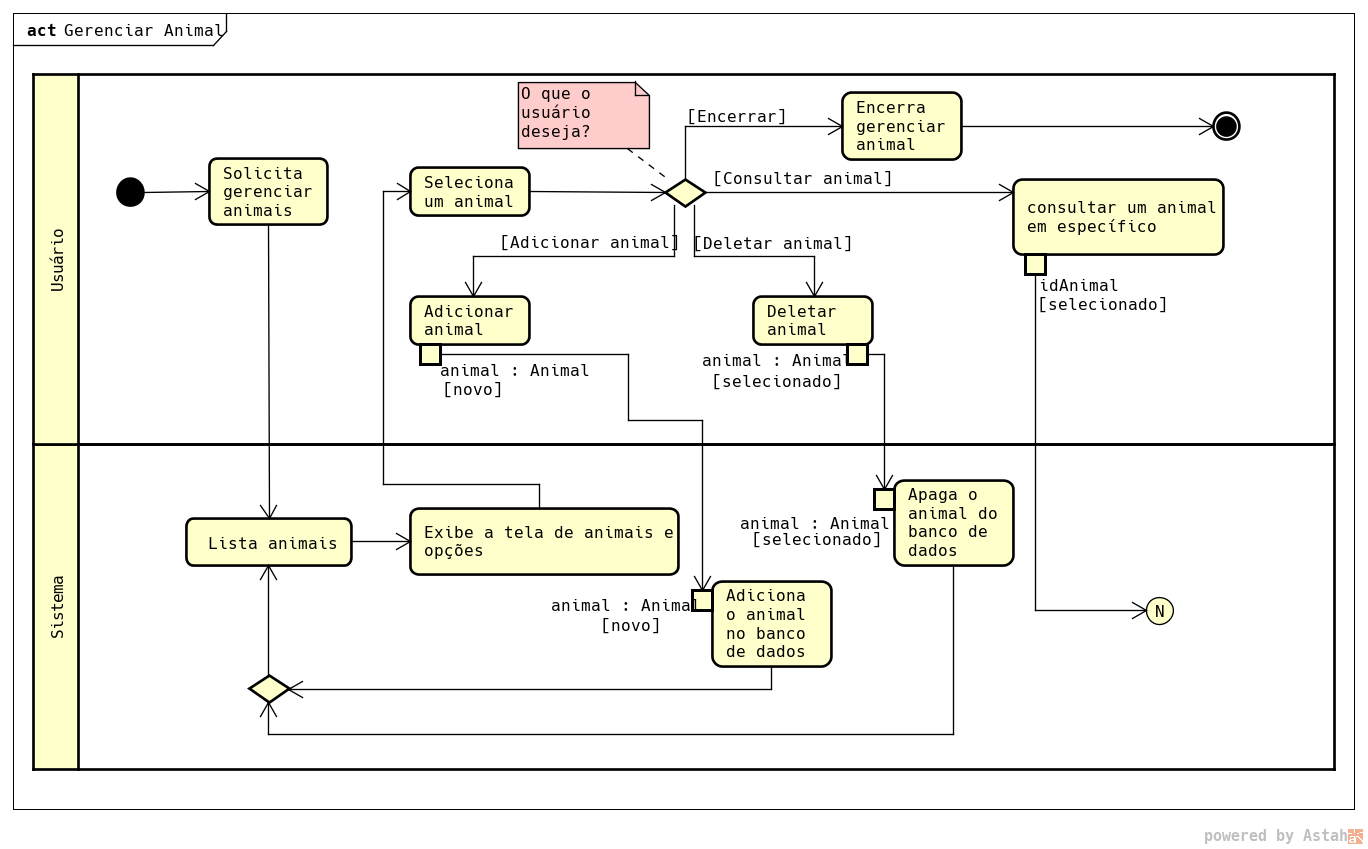
\includegraphics[width=\textwidth]{../img/GerenciarAnimal1.png}

		Fonte: Autoria própria.
	\end{center}
\end{figure}

\begin{figure}[H]
	\begin{center}
		\caption{Diagrama da Atividade de Gerenciar Animal parte 2}
		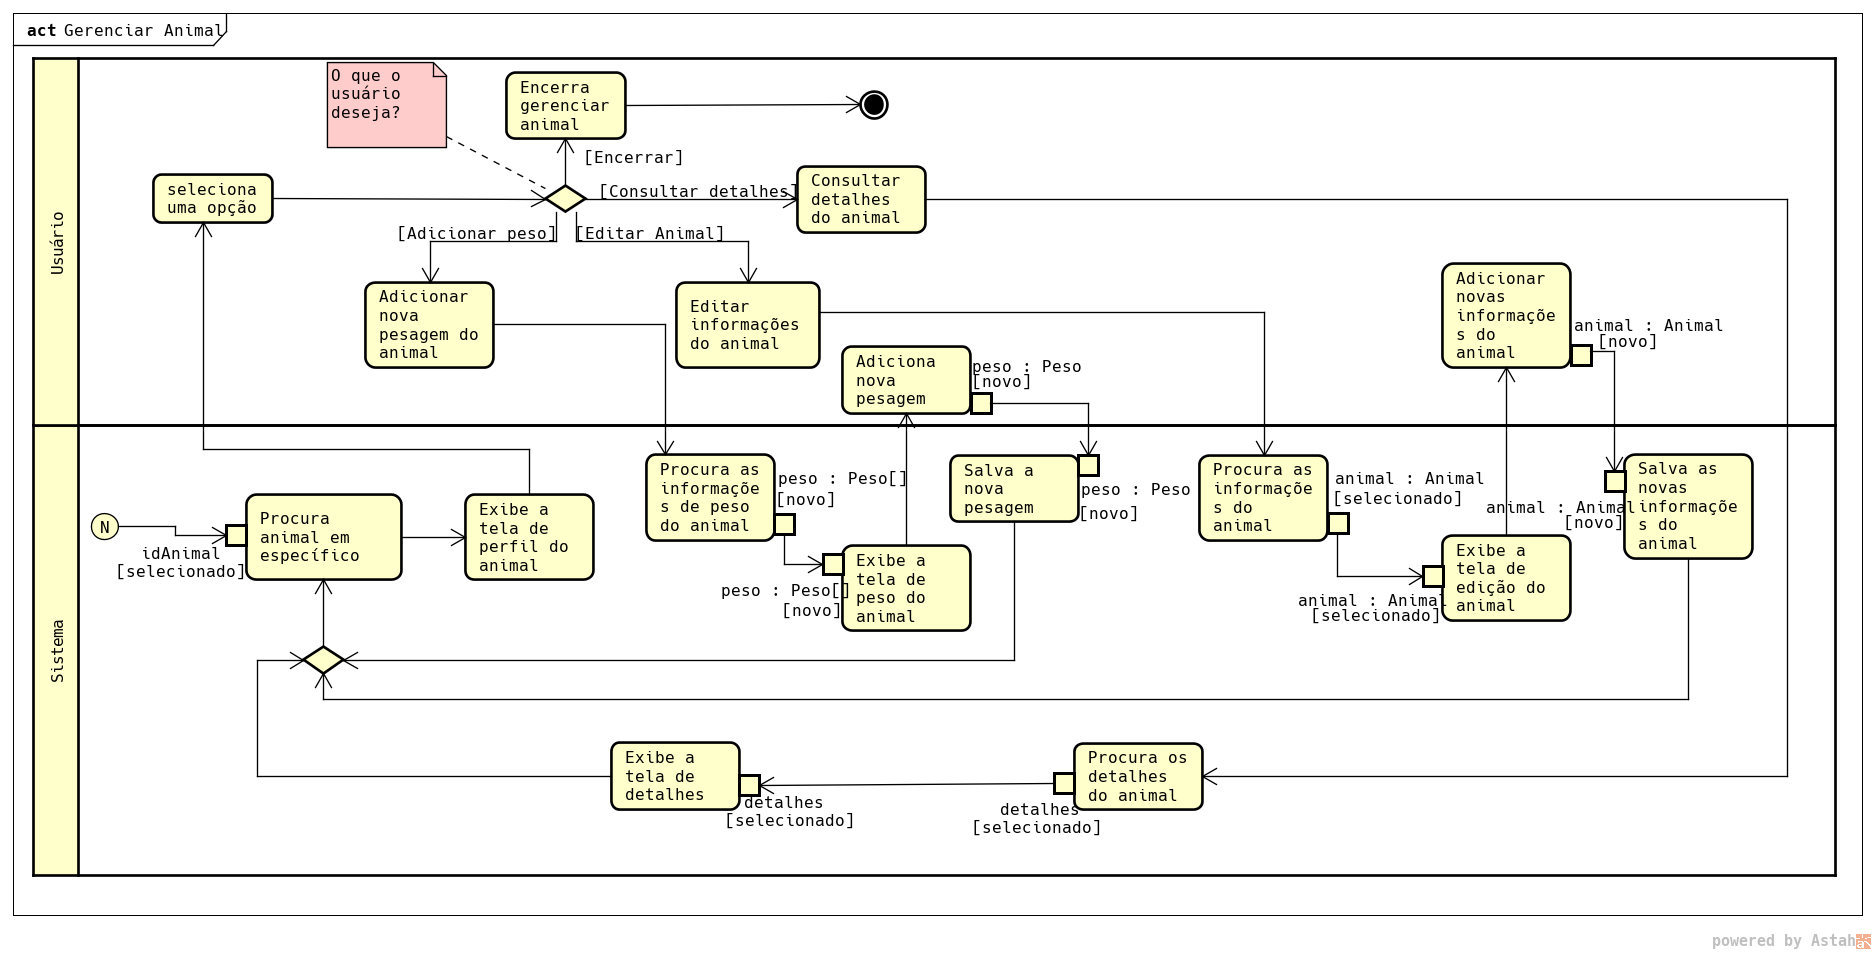
\includegraphics[width=\textwidth]{../img/GerenciarAnimal2.png}

		Fonte: Autoria própria.
	\end{center}
\end{figure}

\begin{figure}[H]
	\begin{center}
		\caption{Diagrama da Atividade de Gerenciar Remédios}
		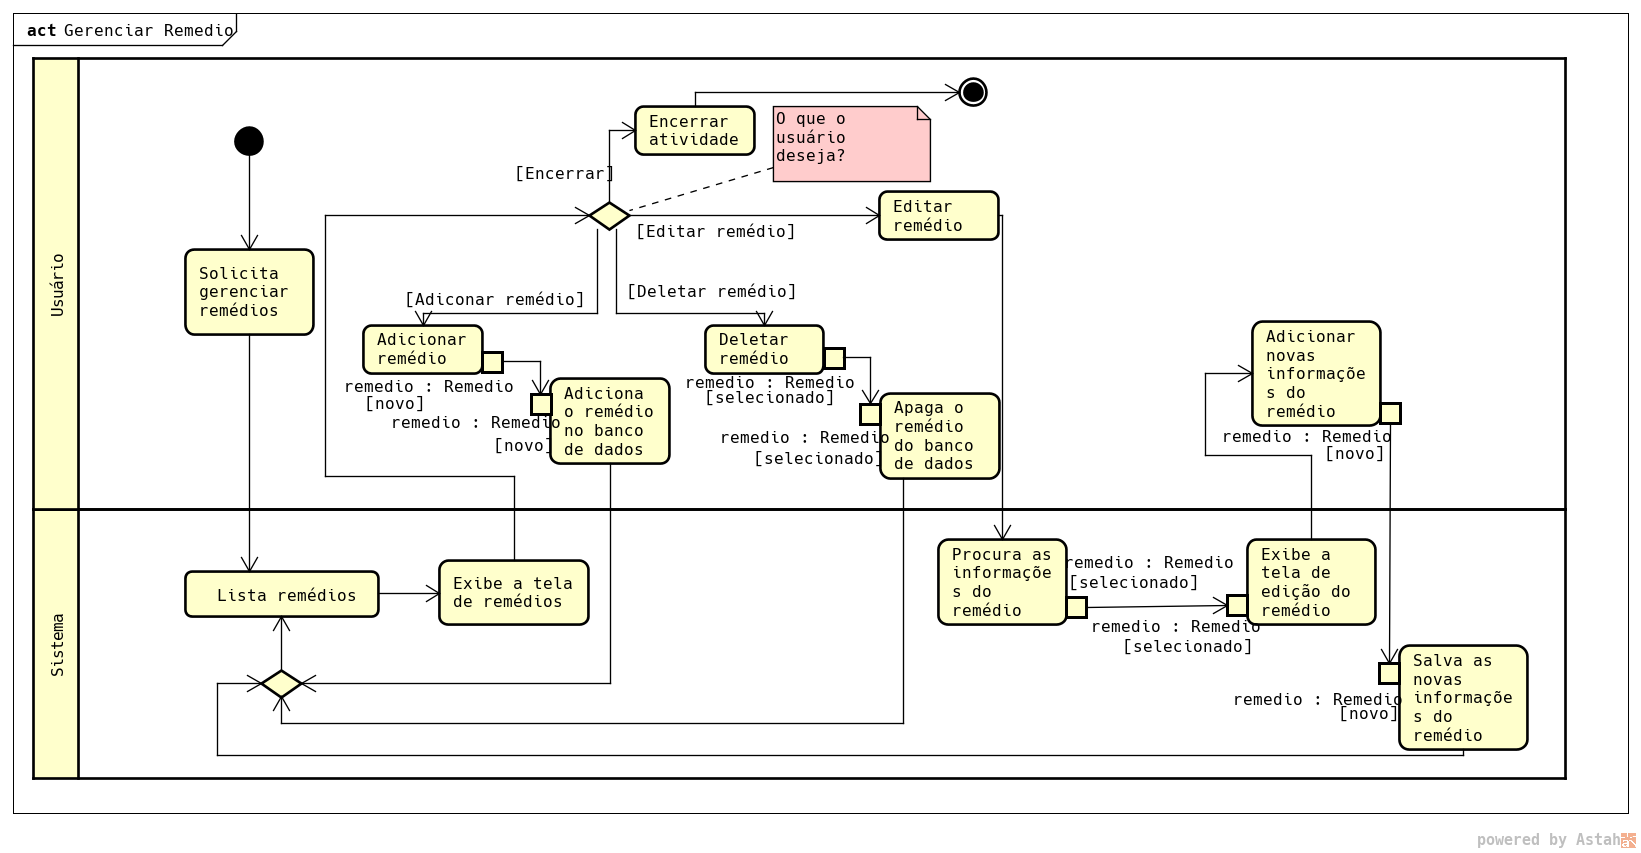
\includegraphics[width=\textwidth]{../img/GerenciarRemedio.png}

		Fonte: Autoria própria.
	\end{center}
\end{figure}

\begin{figure}[H]
	\begin{center}
		\caption{ Diagrama da Atividade de Gerenciar Medicações}
		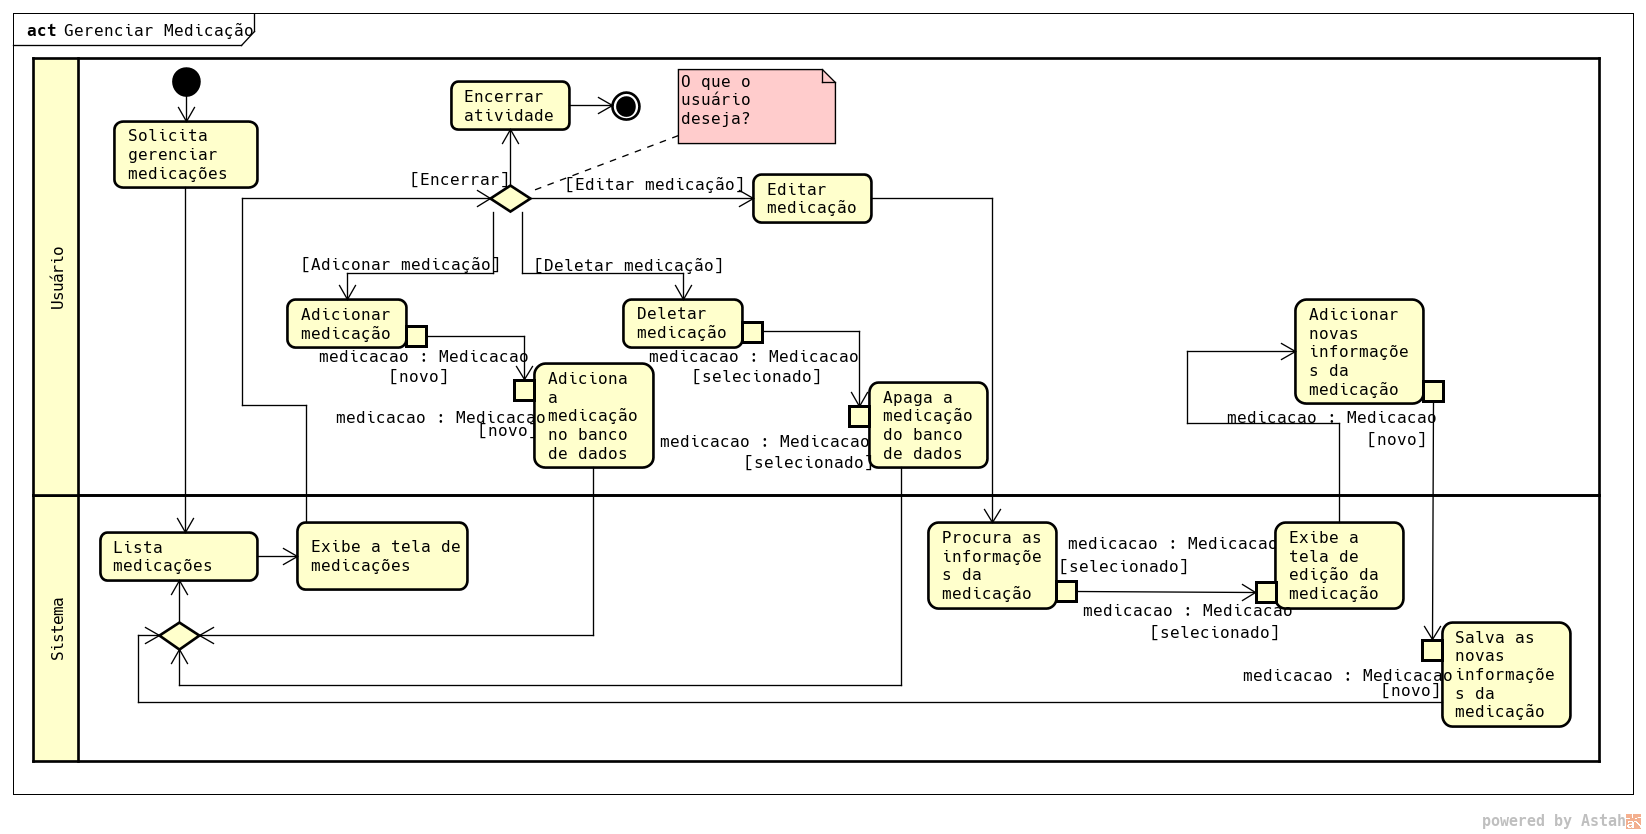
\includegraphics[width=\textwidth]{../img/GerenciarMedicacao.png}

		Fonte: Autoria própria.
	\end{center}
\end{figure}

\begin{figure}[H]
	\begin{center}
		\caption{Diagrama da Atividade de Visualizar Relatórios}
		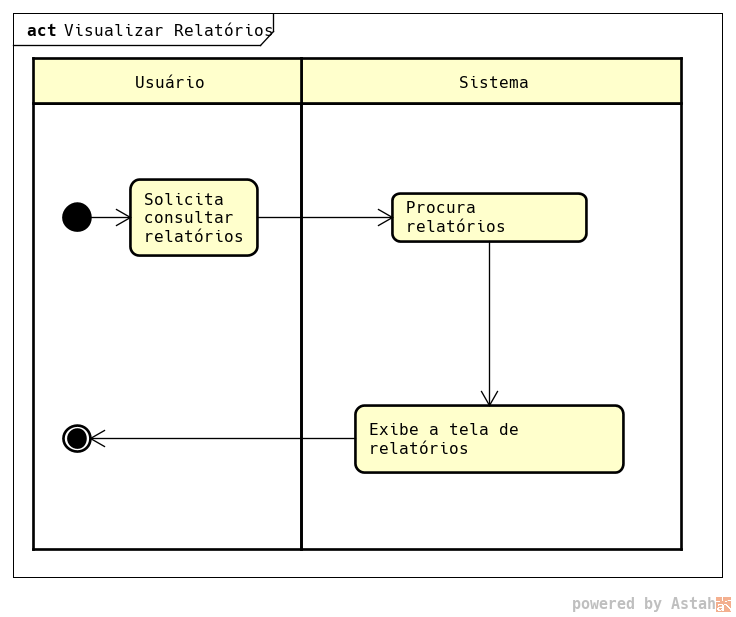
\includegraphics[width=\textwidth]{../img/Relatorios.png}

		Fonte: Autoria própria.
	\end{center}
\end{figure}

\end{apendicesenv}
          % Apêndices
    %\printindex                                             % Índice remissivo

\end{document}
